\documentclass[a4paper,11pt,uplatex]{jsbook}
%\usepackage{fancyhdr}
\setlength{\footskip}{16pt}
\usepackage{amsmath}
\usepackage[dvipdfmx]{graphicx}
\usepackage[dvipdfmx]{color}
%\usepackage{pagecolor}[white]
\usepackage{amsmath,amssymb}
%\usepackage[top=3cm, bottom=3cm, left=3cm, right=3cm]{geometry}
\usepackage{braket}
\usepackage{bm}
\numberwithin{equation}{section}
\usepackage{mathrsfs}
\usepackage{siunitx}
\usepackage{physics}
\usepackage[dvipdfmx]{graphicx}
\usepackage[compat=1.1.0]{tikz-feynhand}
\usepackage{caption}
\usepackage{subcaption}
%\usepackage{cleveref}
\usepackage{float}
\usepackage{multicol}
\setlength{\columnsep}{15mm}
%\usepackage[style=phys,articletitle=false,biblabel=brackets,chaptertitle=false,pageranges=false]{biblatex}
%\usepackage[style=phys]{biblatex}
\usepackage[dvipdfmx]{hyperref}
\usepackage{url}
\usepackage{pxjahyper}
\usepackage{bookmark}
%\usepackage[backref]{hyperref}
\setcounter{tocdepth}{3}
\setlength{\parindent}{2em}
\def\vector#1{\mbox{\boldmath $#1$}}
\def\slash#1{\not\!#1}
\def\slashb#1{\not\!\!#1}
\def\delsla{\not\!\partial}
%\usepackage[dvipdfmx]{xcolor}


\hypersetup{
 setpagesize=false,
 bookmarksnumbered=true,%
 bookmarksopen=true,%
 colorlinks=true,%
 linkcolor=black,
 citecolor=red,
 urlcolor=black,
}
%backreferenceのカスタマイズ. "Back to p.3"のように表示する.
%\renewcommand*{\backref}[1]{(p.#1へ戻る)}
%\newcommand{\backtoc}{\hyperlink{toc}{[目次へ]}}
\newcommand{\backtoc}{\texorpdfstring{\protect\hyperlink{toc}{\hspace{5pt} \scriptsize [目次へ]}}{}}
\newcommand{\mychapter}[1]{\chapter[#1]{#1\backtoc}}
\newcommand{\mysection}[1]{\section[#1]{#1\backtoc}}
\newcommand{\mysubsection}[1]{\subsection[#1]{#1\backtoc}}

% 数式
%\usepackage{amsmath,amsfonts}
%\usepackage{bm}
%\usepackage{physics}
% 画像
%\usepackage[dvipdfmx]{graphicx}
%\usepackage[dvipdfmx,colorlinks=true,linkcolor=blue]{hyperref}
%\usepackage{pxjahyper}

\begin{document}

\chapter{データ解析と結果}\label{ana}
この章ではデータ解析の手順と結果について述べる。

単独アンジュレータのデータおよびエネルギー測定用の2台のアンジュレータのデータの2つのデータセットがある。
画像処理までの手順は共通であるのでまずは画像処理について述べる。
続いて単独アンジュレータのデータの解析結果を述べる。
最後に2台のアンジュレータのデータの解析結果について述べる。\\
なおエネルギー測定のデータセットは以下のように構成されている。
\begin{itemize}
  \item 水銀灯の波長較正データ1枚 (図\ref{beamtime}水銀灯による波長較正を参照)
  \item アンジュレータの位置データ 166個の値
  \item 干渉光の画像データ 166 position $\times$ 4 画像 = 664枚
\end{itemize}
これを反映し、エネルギーデータ解析の手順は以下のようになる。
\begin{enumerate}
  \item 波長較正:ピクセル-波長直線を求める
  \item 画像の統合:664枚$\rightarrow$ 166枚の二次元データ
  \item 較正波長でのデータの切り出し:166枚の二次元データ $\rightarrow$ 166個の1次元データ
  \item モデル関数によるフィッティング
\end{enumerate}

\section{画像処理}
\noindent \textbf{\underline{解析}}\par
各ピクセルにおける発光量に対応して、0から65535(16~bit)の整数値が割り当てられる。この値をピクセル値と定義する。

まず電子ビームを入射していない状態の画像を取得し、これを背景画像とする。露光時間1 秒で10枚の画像を連続で取得し、各ピクセルごとにピクセル値の平均値を計算し、背景画像とする。

各runでは、各ピクセルごとに同一条件(アンジュレータ位置、波長などの条件)で4枚の画像が取得される。
これらの4枚の画像について、各ピクセルごとにピクセル値の平均値を取り、代表値とする。
またピクセルの誤差は4枚の画像におけるピクセル値の標準偏差とする。

予想される回折パターンの性質を考えると、隣り合うピクセル同士の発光量の差は小さい滑らかなパターンになると考えられる。
したがって周囲の上下左右のピクセルに対して極端に発光量が多いピクセルはノイズであると判断してマスクし、フィッティングの対象に含まない。

\noindent \textbf{\underline{結果}}\par
あるピクセルにおける、4枚の画像のピクセル値の平均値と標準偏差の関係を図\ref{pixel}に示す。
\begin{figure}[h]
  \centering
  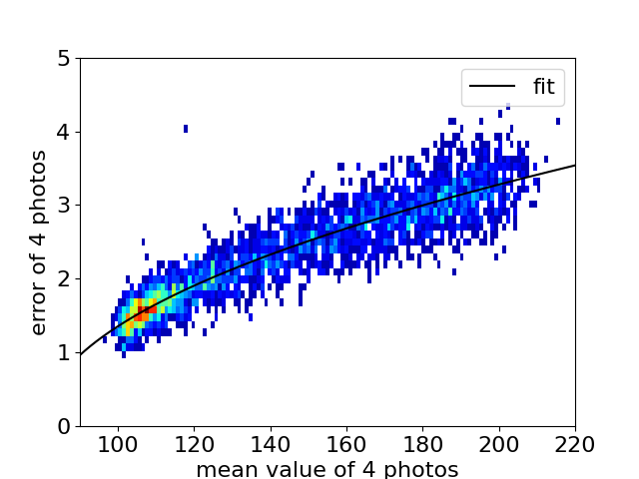
\includegraphics[width=0.8\linewidth]{image/4-pixel.png}
  \caption{ピクセルの平均値と標準偏差の関係}\label{pixel}
\end{figure}

ピクセルの発光量はポアソン分布に従うことから、標準偏差は平均値の平方根に比例すると考えられる。
オフセットを考慮してフィッティングした結果、平均値と標準偏差の関係は
\begin{eqnarray}
  \text{標準偏差} = 0.298(4) \sqrt{\text{平均値} - 79.2(1.6) } 
\end{eqnarray}
となった。

背景画像の結果を図\ref{BG}に示す。発光量が極端に多いノイジーなピクセルが見られるが、ピクセル値が150以上のピクセルは150に置き換えて表示している。
\begin{figure}[H]
  \centering
  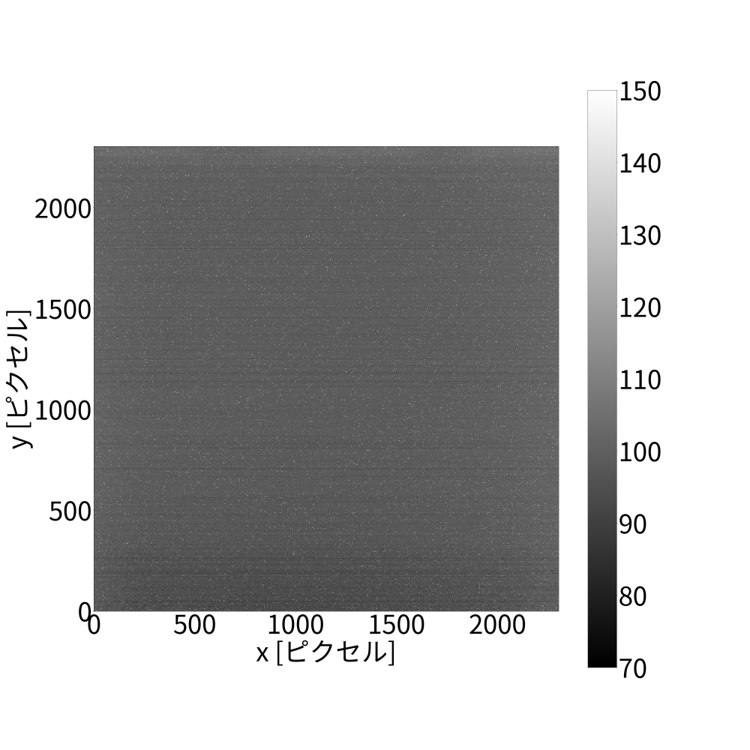
\includegraphics[width=0.8\linewidth]{image/4-BG.png}
  \caption[背景画像]{背景画像。ピクセル値が150以上のピクセルは150に置き換えて白で表示している。}\label{BG}
\end{figure}

背景画像のピクセル値の分布を図\ref{BGmean}に示す。全画素にわたるピクセル値の平均値は98.91、標準偏差は4.57であった。ピクセル値が150以上のピクセルは全体の0.14 \%であった。
\begin{figure}[H]
  \centering
  \begin{subfigure}[b]{0.45\linewidth}
    \centering
    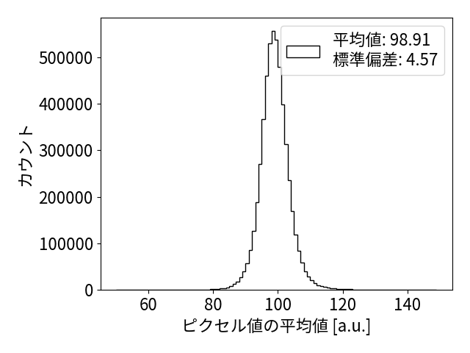
\includegraphics[width=\linewidth]{image/4-BGmean.png}
    \subcaption{150以下の平均値分布}
  \end{subfigure}
  \hfill
  \begin{subfigure}[b]{0.45\linewidth}
    \centering
    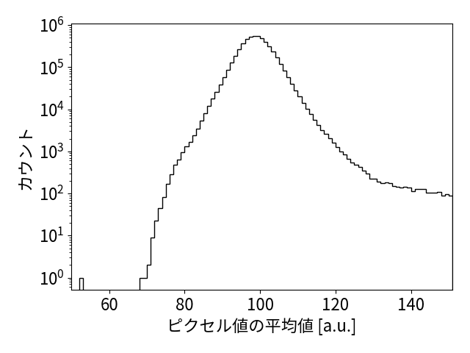
\includegraphics[width=\linewidth]{image/4-BGmeanlog.png}
    \subcaption{150 以下の平均値分布(対数表示)}
  \end{subfigure}
  \hfill
  \begin{subfigure}[b]{0.45\linewidth}
    \centering
    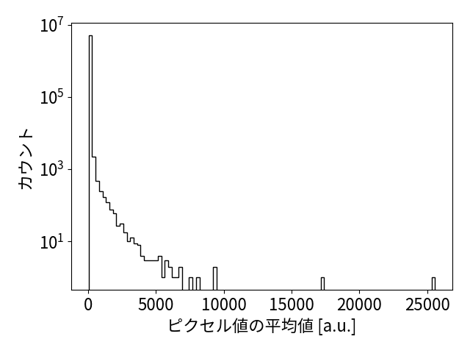
\includegraphics[width=\linewidth]{image/4-BGmeanall.png}
    \subcaption{平均値の全分布}
  \end{subfigure}
  \caption[背景画像の光量分布]{背景画像のピクセルの平均値分布}\label{BGmean}
\end{figure}

周囲のピクセルと比較した超過値の分布を示す(図\ref{excess})。
閾値として40を設定し、閾値を超えるピクセルはノイズピクセルとして除去した。
ノイズピクセルと判定されたピクセルの割合は0.22\%であった。
\begin{figure}[H]
  \centering
  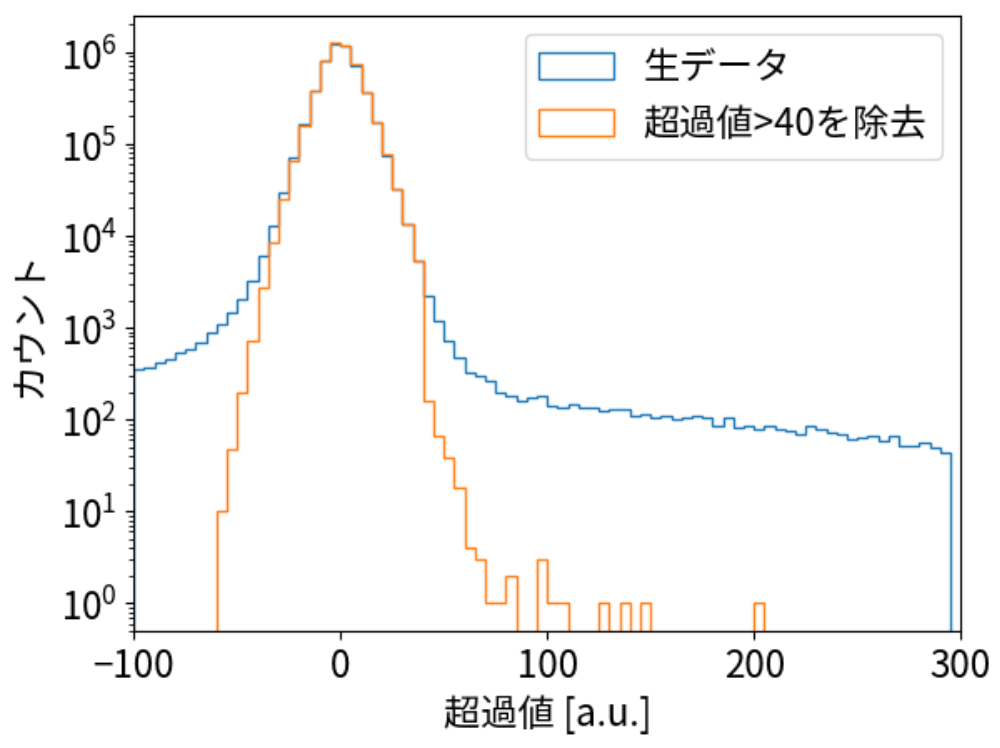
\includegraphics[width=0.5\linewidth]{image/4-excess.png}
  \caption[超過値の分布]{周囲のピクセルと比較した超過値の分布。超過値が40を超えたピクセルを除去する前後の結果を示す。}\label{excess}
\end{figure}
\subsection{平滑化}
画像の平滑化が必要な場合には、波長方向($x$方向)にのみ行う。同様にノイズピクセルをマスクしたうえで、マスクされなかったピクセルの平均値と標準偏差を計算し、ピクセルの誤差は標準偏差を計算に用いたピクセルの数の平方根で割った値(標準誤差)とする。

\section{波長較正}
\noindent \textbf{\underline{解析}}\par
水銀灯の404.656 nmおよび407.781 nmの輝線スペクトルを取得する。画像の$y$軸方向に50 ピクセルのカットをかけた1次元データを取得し、ガウシアンによるフィッティングを行う。
フィッティングで得られたピークの中心値と波長から、ピクセル-波長関係を求める。
ピークの中心決定精度から波長較正の精度を求める。

\noindent \textbf{\underline{結果}}\par
水銀灯の波長較正で得られた画像の例を図\ref{mercury}に示す。
\begin{figure}[h]
  \centering
  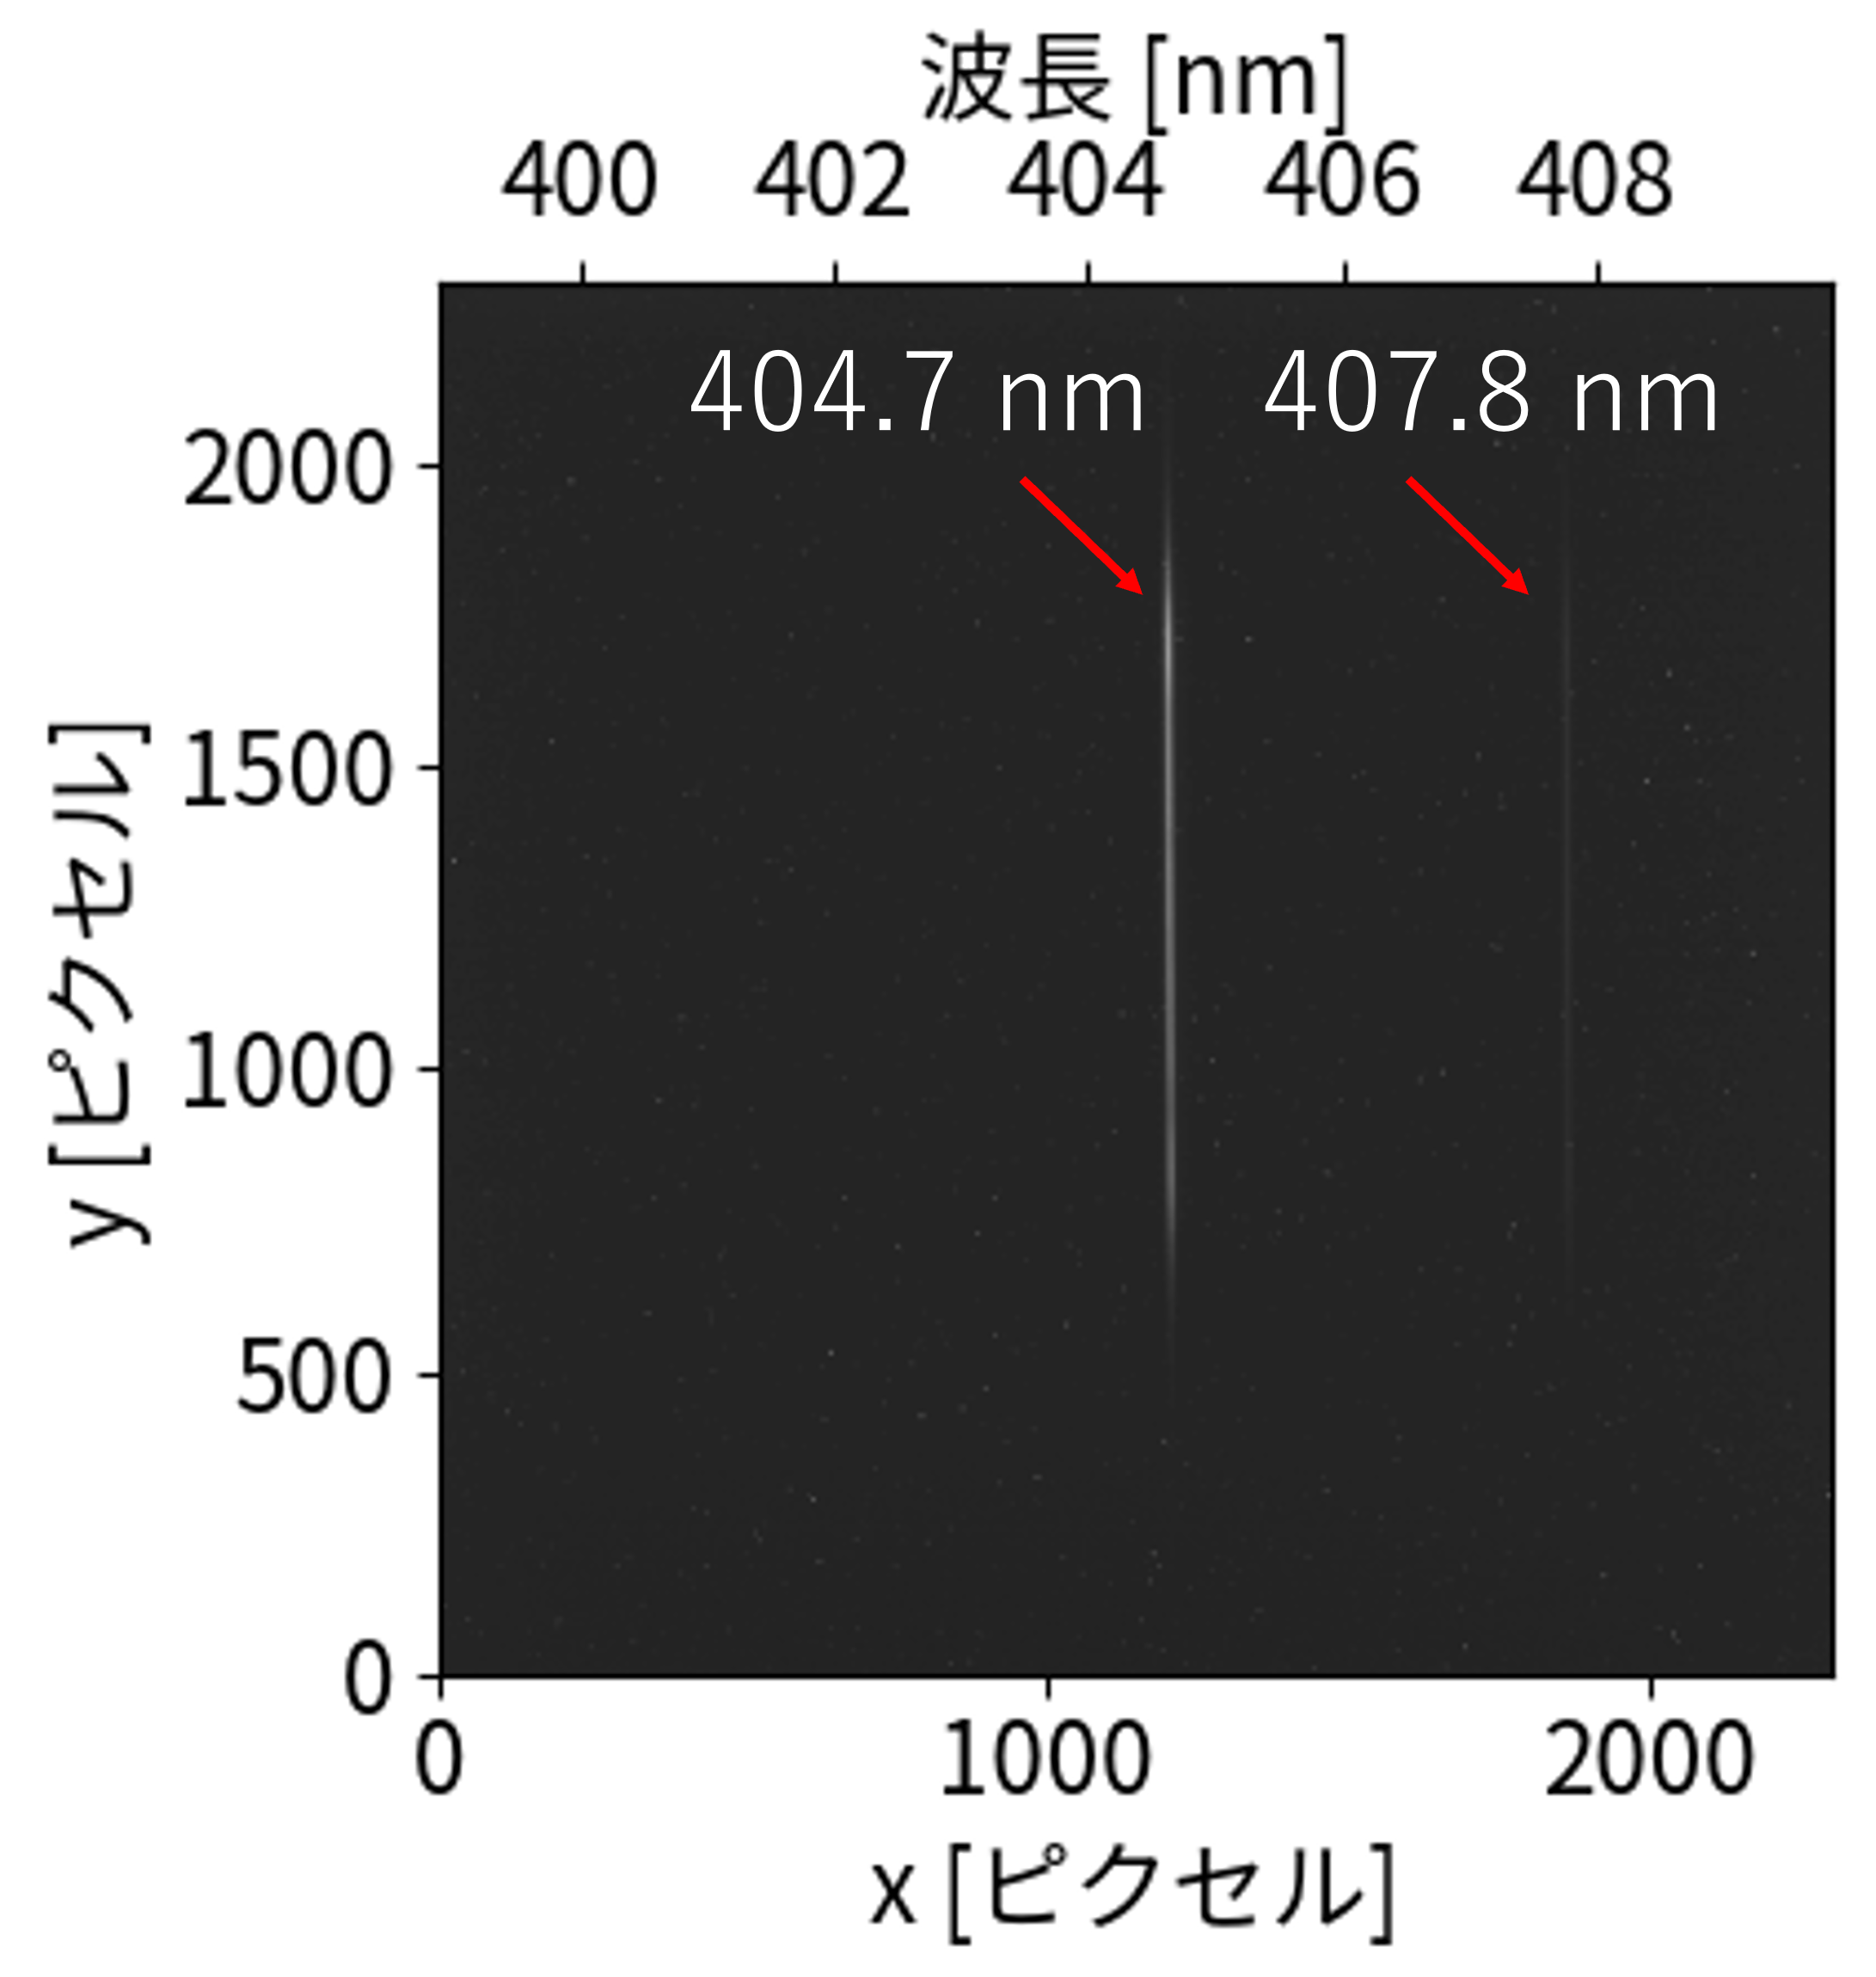
\includegraphics[width=0.6\linewidth]{image/4-mercury.png}
  \caption[水銀灯の波長較正-1]{水銀灯の波長較正で得られた画像。404.656 nmと407.781 nmに対応する輝線が見える。この輝線スペクトルをもとにピクセル$-$波長関係から得られた波長の値が画像の上の軸である。}\label{mercury}
\end{figure}
$y$軸方向に50 ピクセルのカットをかけて、ガウシアンによるフィッティングを行った結果を図\ref{mercuryfit}に示す。
輝線スペクトルの中心付近でのカットの結果、中心値のピクセルとフィットによる中心決定精度は
\begin{eqnarray}
  ピクセル_{404.7} &=& 1209.5912(9)\\
  ピクセル_{407.8} &=& 1868.155(4) 
\end{eqnarray}
と求められた。これらの値を元に、ピクセル$-$波長関係が求められる。特に1 ピクセルあたりの波長分散は、
\begin{eqnarray}
  \lambda_L / ピクセル = 0.0047~\text{nm}
\end{eqnarray}
である。また、輝線スペクトルの幅($\sigma$)は404.656 nmのピークが3.5 ピクセル、407.781 nmのピークが2.1 ピクセルと見積もられているが、これはそれぞれ0.0016 nm、0.0010 nmの波長分散に相当し、
較正波長約400 nm に対して$10^{-4}$以下に抑えられている。
\begin{figure}[H]
  \centering
  \begin{subfigure}[h]{0.45\linewidth}
    \centering
    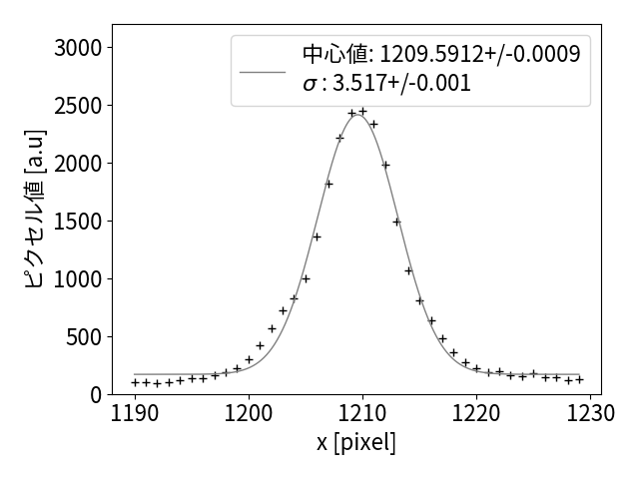
\includegraphics[width=\linewidth]{image/4-fpeak.png}
    \subcaption{404.656 nmのピーク}
  \end{subfigure}
  \hfill
  \begin{subfigure}[h]{0.45\linewidth}
    \centering
    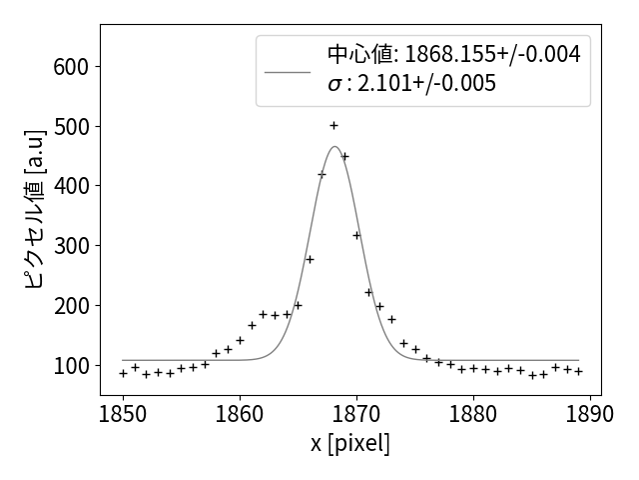
\includegraphics[width=\linewidth]{image/4-speak.png}
    \subcaption{407.781 nmのピーク}
  \end{subfigure}
  \hfill
  \begin{subfigure}[h]{0.45\linewidth}
    \centering
    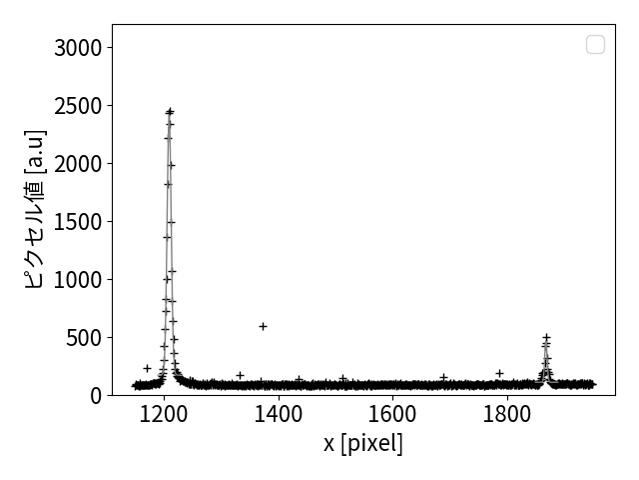
\includegraphics[width=\linewidth]{image/4-bothpeak.png}
    \subcaption{2つのピーク}
  \end{subfigure}
  \caption[水銀灯の波長較正-2]{水銀灯のデータをガウシアンでフィッティングした結果。フィッティングパラメータの中心値および標準偏差$\sigma$の結果を判例に示した。これらの数値に付けられている誤差はフィッティングの誤差を表す。}
\label{mercuryfit}
\end{figure}

次に水銀灯の輝線がカメラに対してどの程度傾いているかを調べた。
$y$軸方向のカットをかけるピクセルを輝線が明瞭に見える$y$ = 700 ピクセルから$y$ = 1800 ピクセルの範囲で変えてガウシアンフィッティングを行い、ピークの中心値の依存性を調べた結果を図\ref{tiltfit}に示す。
2つのピークで中心値の傾きは線形で近似可能であり、これは光軸に対してカメラが傾いている効果で説明可能である。
またその傾きは線形フィットによれば
\begin{eqnarray}
  x方向の変位 / y軸方向の変位 = 5 \times 10^{-3}
\end{eqnarray}
程度に抑えられており、カメラの上下2304 ピクセルに対して約12ピクセルの変位が生じることがわかる。
1ピクセルあたりの波長分散は0.0047~nmであるからこれは0.05~nmに相当する。
しかし、発光量の多い領域は高々1500 ピクセル程度の範囲に限られており、この領域における波長分散は最大0.035~nm程度と見積もられる。
式(\ref{zero order energy formula}) $E_{beam} =m_e c^2  \sqrt{\lambda_{\text{osc}}/2\lambda_L} $によって、波長決定精度がエネルギー決定精度に与える影響を見積もると、$\delta E_beam/E_beam = \delta \lambda_L/\delta \lambda_L$であり、
ここに較正波長$\lambda_L \sim 400~\text{nm}$、$\delta \lambda_L \sim 0.0035~\text{nm}$を代入すれば
カメラの傾きによる波長分散の効果は$10^{-4}$以下に抑えられていると言える。
\begin{figure}[H]
  \centering
  \begin{subfigure}[h]{\linewidth}
    \centering
    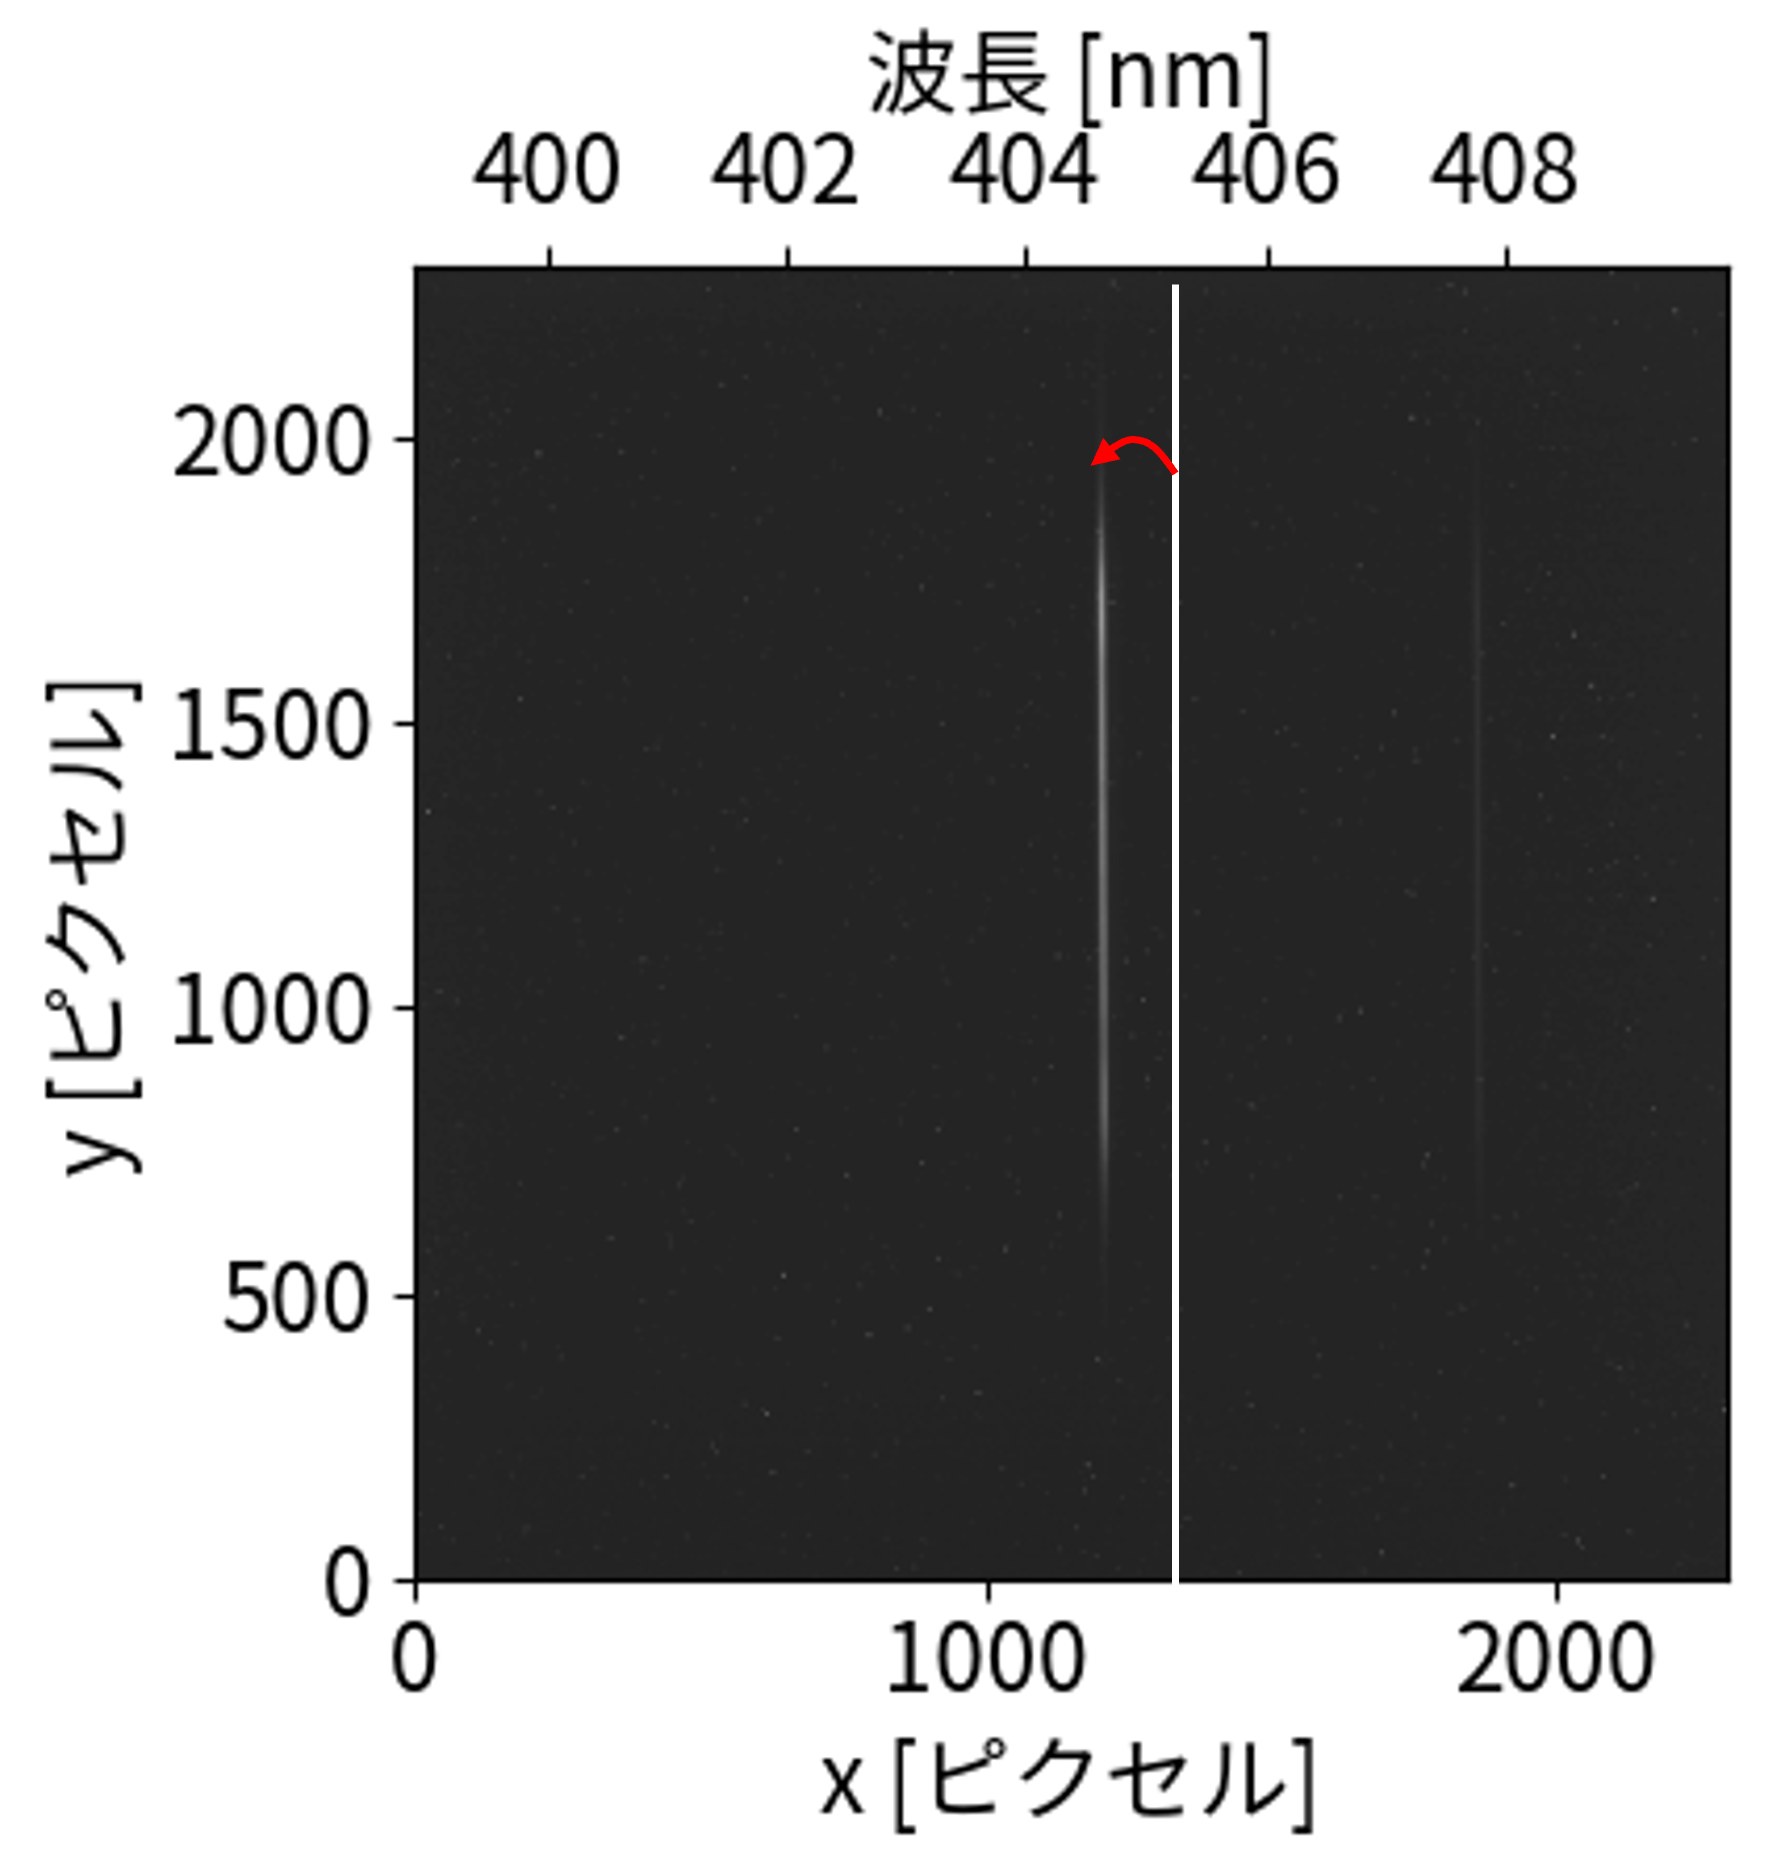
\includegraphics[width=\linewidth]{image/4-tilt.png}
    \subcaption{輝線の傾きの図示}
  \end{subfigure}
  \hfill
  \vspace{1em}
  \begin{subfigure}[h]{0.45\linewidth}
    \centering
    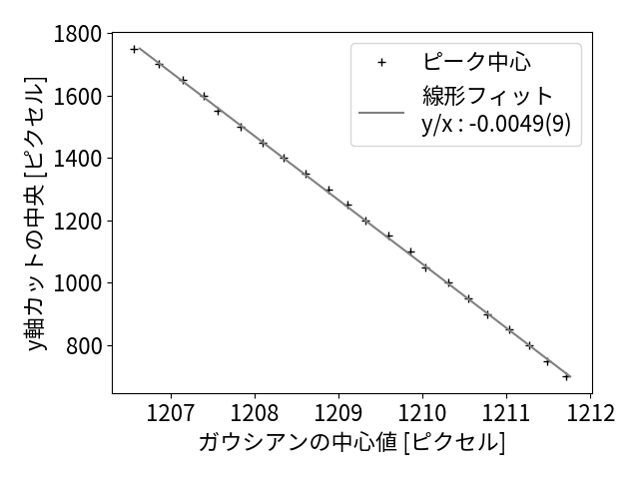
\includegraphics[width=\linewidth]{image/4-tiltfpeak.png}
    \subcaption{404.656 nmのピーク}
  \end{subfigure}
  \hfill
  \begin{subfigure}[h]{0.45\linewidth}
    \centering
    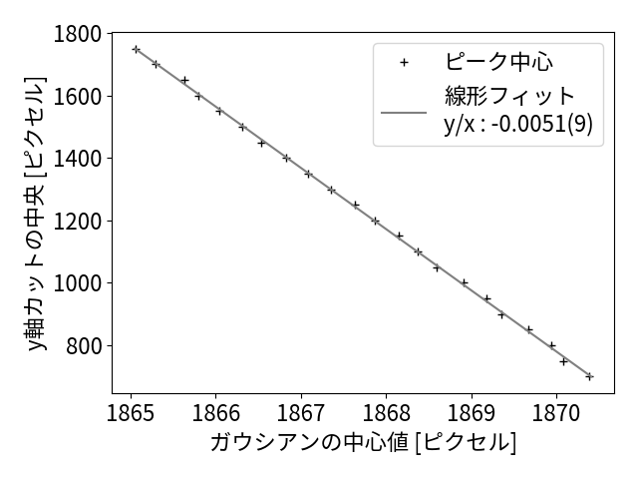
\includegraphics[width=\linewidth]{image/4-tiltspeak.png}
    \subcaption{407.781 nmのピーク}
  \end{subfigure}
  \caption[水銀灯の波長較正-3]{輝線スペクトルの傾きの解析結果。$y$軸方向に50 ピクセルのカットをかける範囲を変えてガウシアンフィッティングを行い、その中心値をプロットした。2つのピークに対して$y$-ガウシアンの中心関係を線形フィットして得られた傾きの値を凡例に示した。}\label{tiltfit}
\end{figure}

\section{モデル関数によるフィッティング}
\noindent \textbf{\underline{解析}}\par
この節では、単独アンジュレータのデータおよび2台のアンジュレータのデータ両方の解析に用いるモデル関数について述べる。
モデル関数は、エネルギーを含む各種パラメータとアンジュレータの位置を入力として、回折パターンの形状をカメラの$y$座標の関数として出力する関数である。


これらの変数の定義を表\ref{tab:variables}に示す。
\begin{table}[h]
  \centering
  \begin{tabular}{c|c}
    $\lambda_L$ & 観測光の波長。波長較正によってカメラの$x$軸と波長の関係が求まる。\\
    $y$ & カメラにおける$y$座標。-7.488 mm から7.488 mmの値をとる。\\
    $d$ & アンジュレータの位置。0(最上流) $\sim$ 825(最下流) mmの値をとる。\\
  \end{tabular}
  \caption[変数の定義]{変数の定義}\label{tab:variables}
\end{table}

また関数の出力を制御するパラメータを表\ref{tab:prm}および図\ref{prm}に示す。上流アンジュレータの位置は固定されているため、
モデル関数で上流アンジュレータの位置パラメータは常に$z(U1-slit)$を用いる。
これに対して可動式の
\begin{table}[h]
  \centering
  \begin{tabular}{c|c|c}
    パラメータ & 意味 & 実測値\\ \hline 
    $\gamma$ & 電子ビームエネルギーのローレンツ因子 & 350,380,410 (目安)\\
    $K$ & アンジュレータの偏向定数 & 0.710, 0.971, 1.046 \ref{undulator_setting}\\
    $\sigma_y$ & ビームサイズ & およそ100~$\mu$m \\
    $z(U1-slit)$ & 上流アンジュレータ-スリット間の距離 & 10.26(10) m(実測値)\\
    $z(U2-slit)$ & 下流アンジュレータ(最上流)-スリット間の距離 & 11.64(10) m(実測値)\\
    $z(slit-cam)$ & スリット-カメラ間の距離 & 4.11(5) m(実測値)\\
    $w(slit)$ & スリットの鉛直方向の長さの1/2 & 3.0(0.2) mm(実測値)\\
    $y(beam)$ & カメラに対するビーム中心の$y$座標 & 数 mm(ビーム状況に依存)\\
    $y(slit)$ & カメラに対するスリット中心の$y$座標 & 数 mm\\
    $\delta d$ & 上流と下流のアンジュレータ放射の位相差オフセット &  -\\
    $ampl$ & 光量にかかる比例係数 & - 
  \end{tabular}
  \caption[パラメータの説明]{パラメータの説明。実測値があるものは値を示した。また、$\gamma$と$K$の3つの値は順に
  180,195,210~MeVの3つのビームエネルギーに対応している。$y(beam),y(slit),\delta d, ampl$の4つのパラメータはビームのコンディションに依存する任意パラメータである。}\label{tab:prm}
\end{table}
  
\begin{figure}[H]
  \centering
  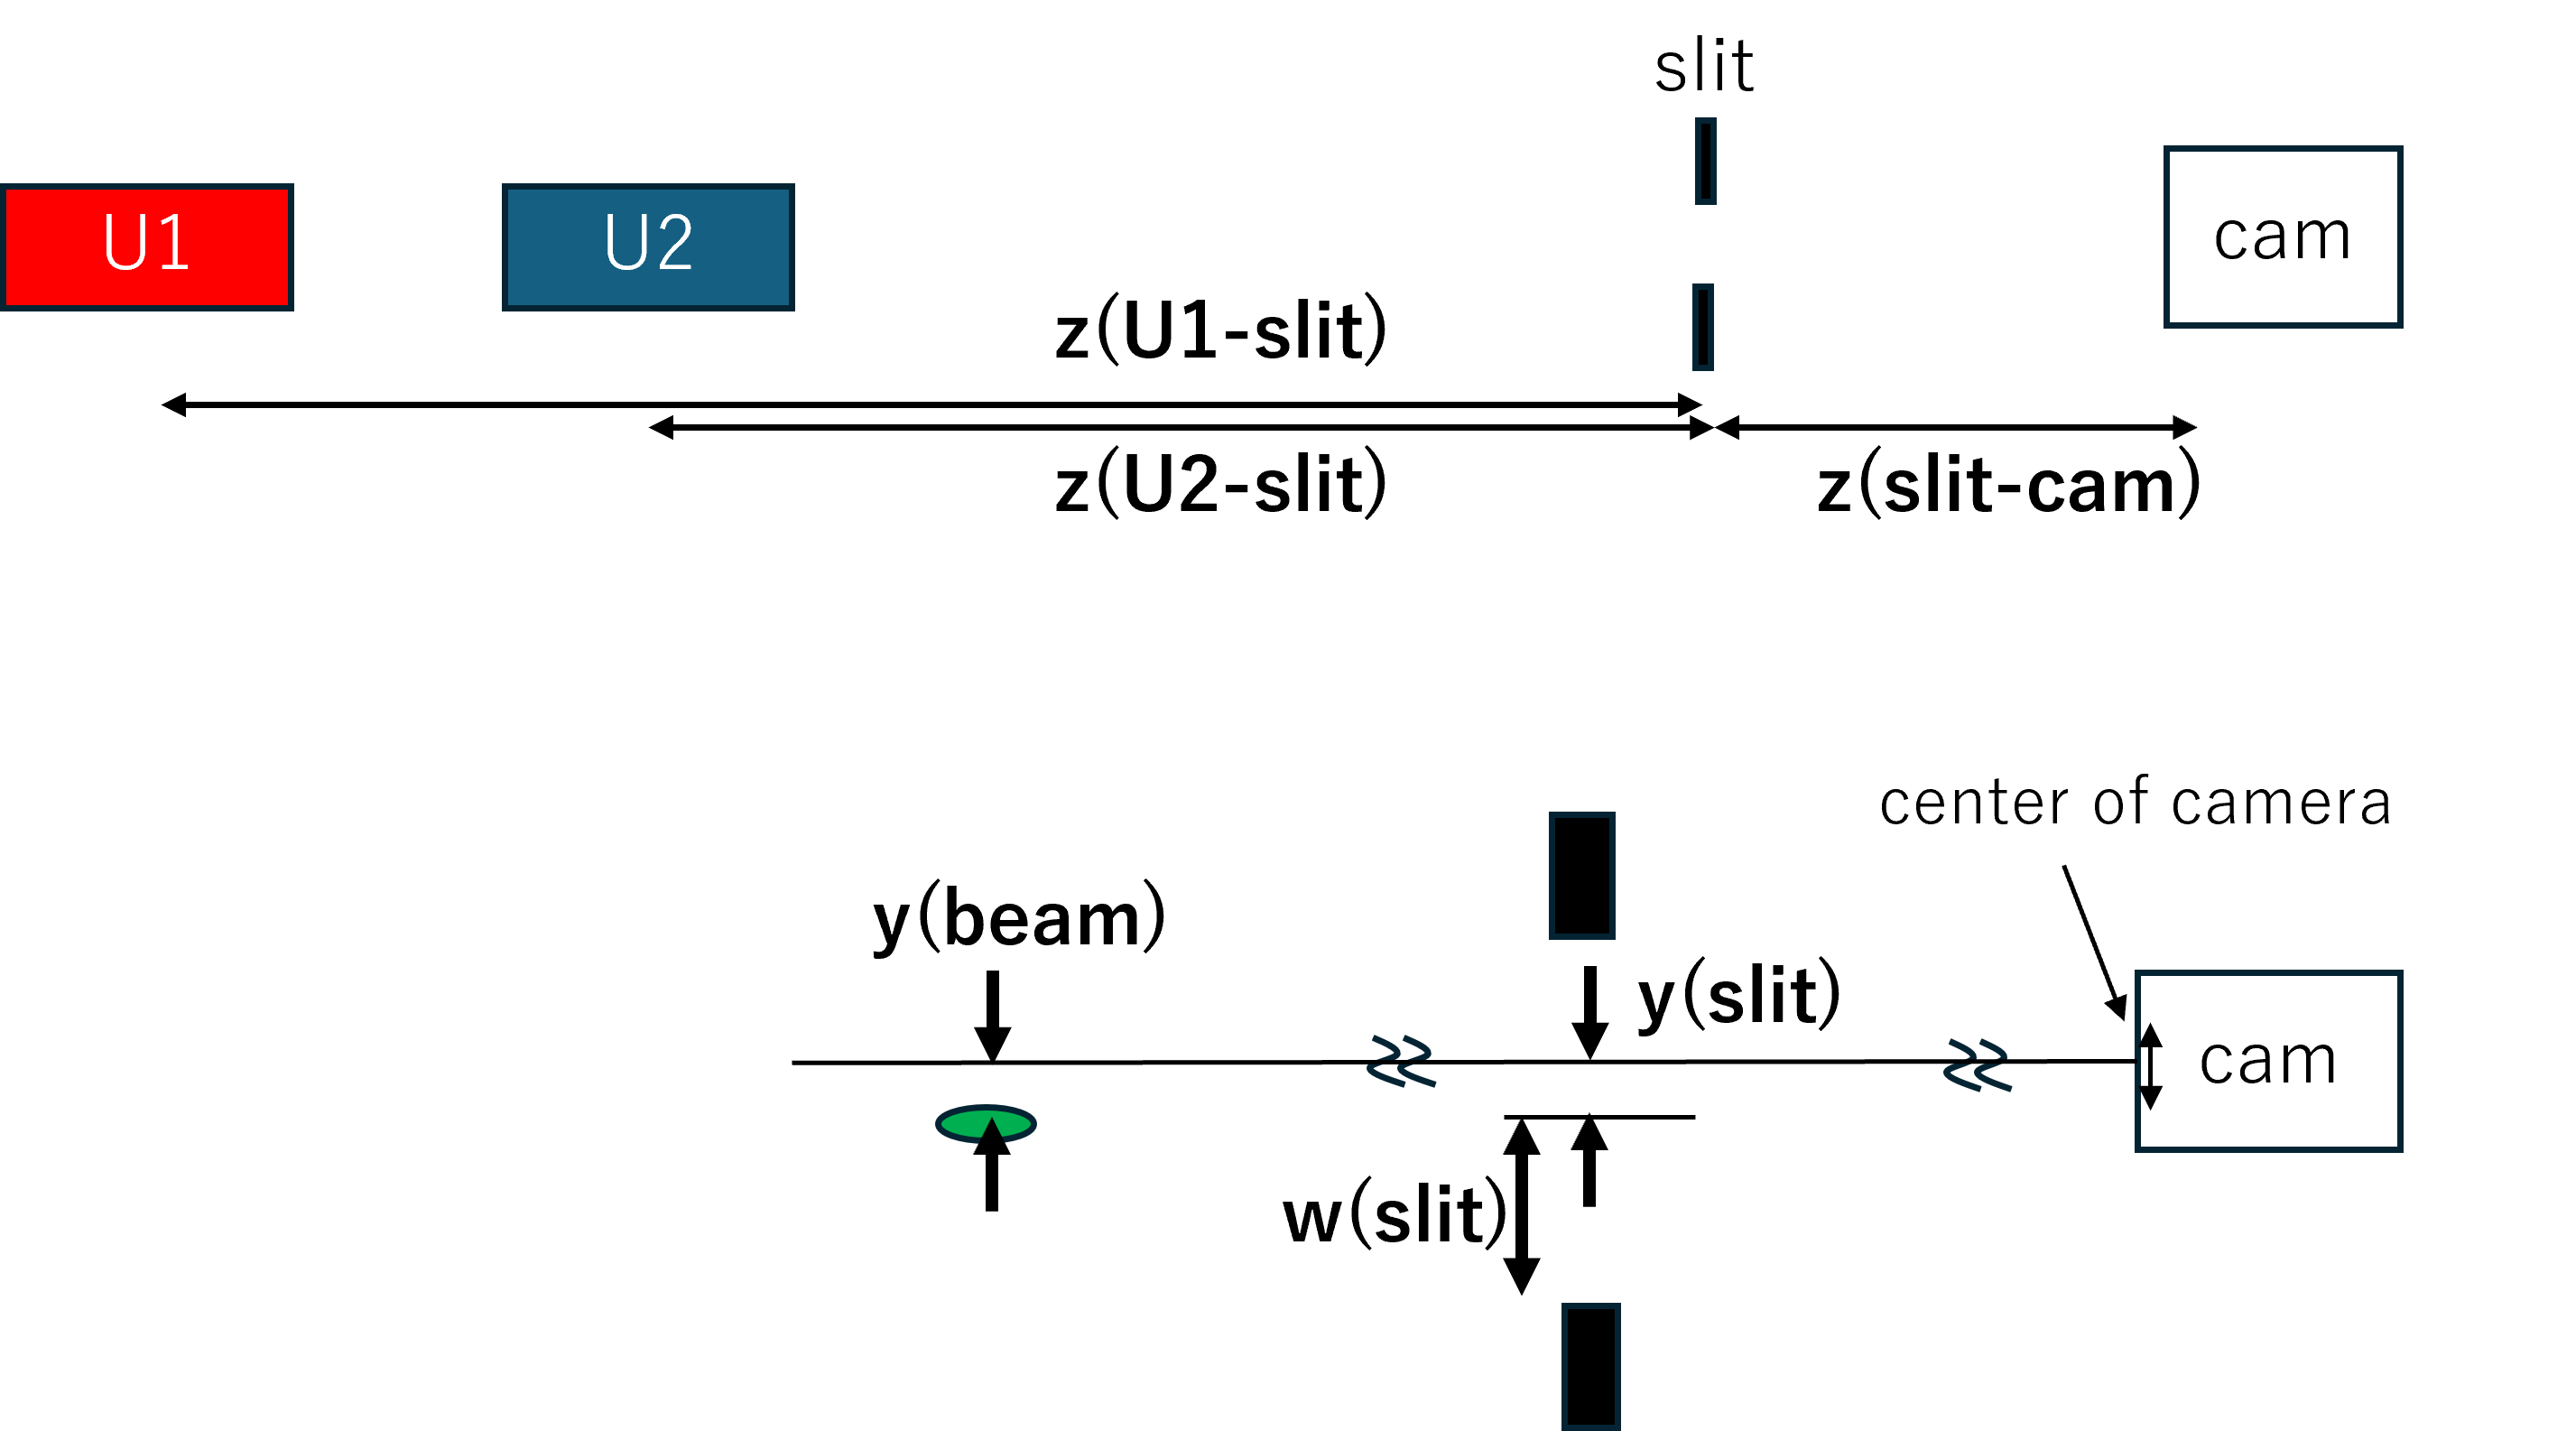
\includegraphics[width=0.8\linewidth]{image/4-prm.png}
  \caption[パラメータの定義]{パラメータの定義。アンジュレータ、光学系、
  ビーム同士の幾何学的な位置関係に関するパラメータを示した。}\label{prm}
\end{figure}

\subsection{放射光関数}
放射光関数は、電子ビームとアンジュレータのパラメータをもとにスリット直前の入射光の電場振幅および位相を計算する。

振幅は式(\ref{eq:spectrum})によって計算される。特にスリット上で$x=0$として計算を行うと、$\phi = \pm\pi/2$であり、 
\begin{align}
  \cos \phi = 0, \sin \phi = \pm 1
\end{align}
また、$\cos \phi = 0$と、ベッセル関数が$J_0(0) = 1, J_{p\ne 0}(0) = 0$であることから、
\begin{align}
  S_0 &= \sum_{p = -\infty}^{\infty} J_{1+2p}(0)J_p(K^2/4)  = 0 \\
  S_1 &= \sum_{p = -\infty}^{\infty} J_{2+2p}(0)J_p(K^2/4)  =  J_{-1}(K^2/4)\\
  S_{-1} &= \sum_{p = -\infty}^{\infty} J_{2p}(0)J_p(K^2/4) = J_0(K^2/4)
\end{align}
したがって$x=0$における放射光の電場振幅は、
\begin{align}
  \frac{\text{d}^2E}{\text{d}\omega \text{d}\Omega} = \frac{e\gamma\xi}{\pi \sqrt{c}}\left| \frac{\sin \{N\pi(\omega/\omega_1 -1)\}}{(\omega/\omega_1 -1)} \right|
  \left| K\left\{ J_1(K^2/4) - J_0(K^2/4) \right\} \right|
\end{align}
という実数関数で与えられる。特に$y$依存性は、$\theta \simeq (y -y(beam))/ z$に依存する$\xi$と$\omega_1$によって決まる。
$y(beam)$による放射光関数の振幅の$y$依存性を図\ref{fig:ybeam}に示す。
\begin{figure}[H]
  \centering
  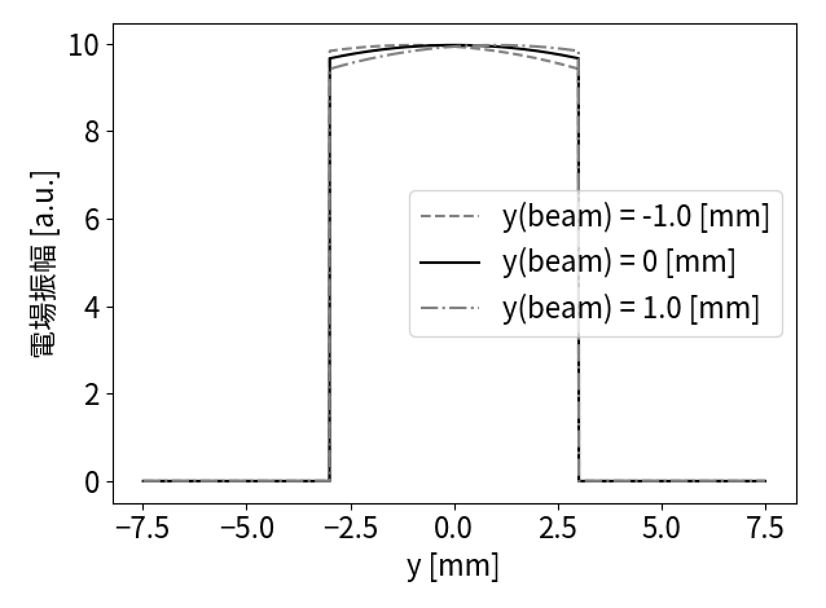
\includegraphics[width = 0.8\linewidth]{image/2-ybeam.png}
  \caption[放射光関数のビーム位置依存性]{放射光関数の振幅の$y(beam)$依存性。$\gamma$= 380, $K$ = 0.971, $z$ = 10.26 mのパラメータで計算した。
  また後述のスリットによる遮蔽の計算が行われている。}
  \label{fig:ybeam}
\end{figure}

電場の位相はアンジュレータの位置を光源とした球面波位相
\begin{align}
  \exp(-ikr) \propto \exp( -ik \frac{(y - y(beam))^2}{z})
\end{align}
を仮定する。球面波位相の導入による放射光関数の実部と虚部を図\ref{fig:phase}に示す。
\begin{figure}[h]
  \centering
  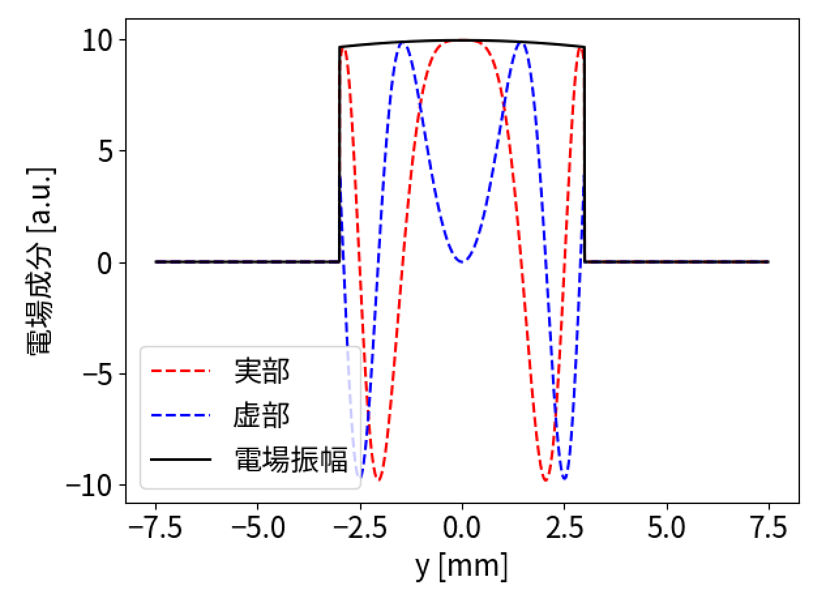
\includegraphics[width=0.8\linewidth]{image/2-phase.png}
  \caption[放射光関数の球面波位相]{放射光関数の球面波位相の導入。$\gamma$= 380, $K$ = 0.971, $z$ = 10.26 mのパラメータで計算した。また後述のスリットによる遮蔽の計算が行われている。}
  \label{fig:phase}
\end{figure}

結局放射光関数の出力は$x=0$においては$y$方向の依存性のみに着目して定数部分を省けば、
\begin{align}
  Rad(x=0, y) \propto \frac{1}{1 + K^2 +\gamma^2\theta^2}\left| \frac{\sin \{N\pi(\omega/\omega_1 -1)\}}{(\omega/\omega_1 -1)} \right| \exp( -ik \frac{(y-y(beam))^2}{z})\\
   \omega_1 = \frac{2\gamma^2\omega_0}{1+ K^2/2+(\gamma \theta^2)}  = \frac{2\gamma^2\omega_0}{1+ K^2/2+(\gamma (y-y(beam))/z)^2} 
\end{align}
このとき、$\lambda_L$は$k = 2\pi/\lambda$の関係にあり、
下流アンジュレータの位置$d$は$z = z(U2-slit) - d $の形で関数に入力される。また、上流アンジュレータの場合には$z = z(U1-slit)$である。

\subsection{電子ビームサイズ}
1電子の放射光であると仮定していた放射光関数は、電子ビームサイズを考慮すると、異なる電子からの放射光関数の重ね合わせとして表現できると考えられる。
$y$軸方向のビームサイズを$\sigma_y$として、電子の位置$y_e$が$y(beam)$を中心としたガウス状の広がり
\begin{align}
  P(y_e) = \exp \left[ -\frac{(y_e - y(beam)^2)}{2\sigma_y^2} \right]
\end{align}
に従うと仮定し、放射光関数を畳みこむ。
これにより1電子放射光関数から得られる回折パターンはぼやける。電子ビームサイズによって回折パターンがぼやける様子を計算で再現した結果を図\ref{beamsize}に示す。
\begin{figure}[H]
  \centering
  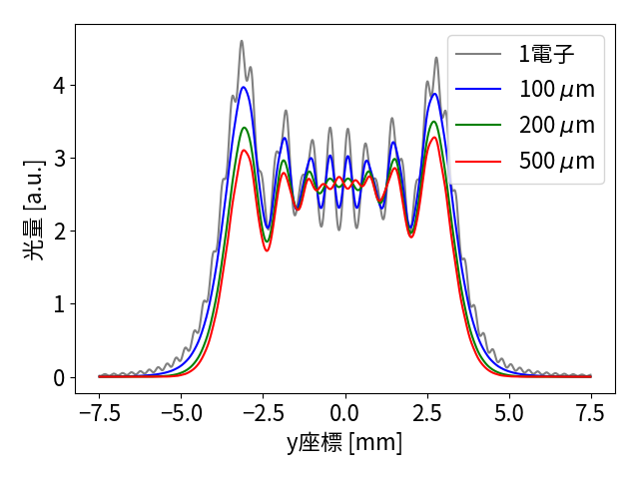
\includegraphics[width=0.8\linewidth]{image/4-esize.png}
  \caption[放射光関数の電子ビームサイズの効果]{電子ビームサイズによる回折パターンのぼやけ。畳み込みがない場合(灰色)と比較して
  ビームサイズの効果を入れた青、緑、赤の線は回折の微細構造がぼやけている}\label{beamsize}
\end{figure}

\subsection{干渉項}
上流と下流の2つのアンジュレータからの放射光の位相差は\ref{sec:interference}節で述べたように$d'/2\gamma^2$と近似できるが、
より厳密にはアンジュレータ内では電子の蛇行運動により$z$軸に沿った平均速度が電子の速度$\beta$よりも小さくなる効果を考慮する必要がある。
この位相差のオフセットを$\delta d$として、干渉光の電場振幅は
\begin{align}
  Rad_{int} &= Rad(y, z(U1-slit)) + Rad(y, z(U2-slit) -d )\exp(i \left[2\pi \frac{d' + \delta d}{2\gamma^2\lambda_L}\right])\\
  d' &= z(U1-slit) - z(U2-slit) + d
\end{align}
と表すことができる。干渉項による放射光関数の変化を図\ref{fig:int}に示す。

\begin{figure}[H]
  \begin{subfigure}[h]{0.45\linewidth}
    \centering
    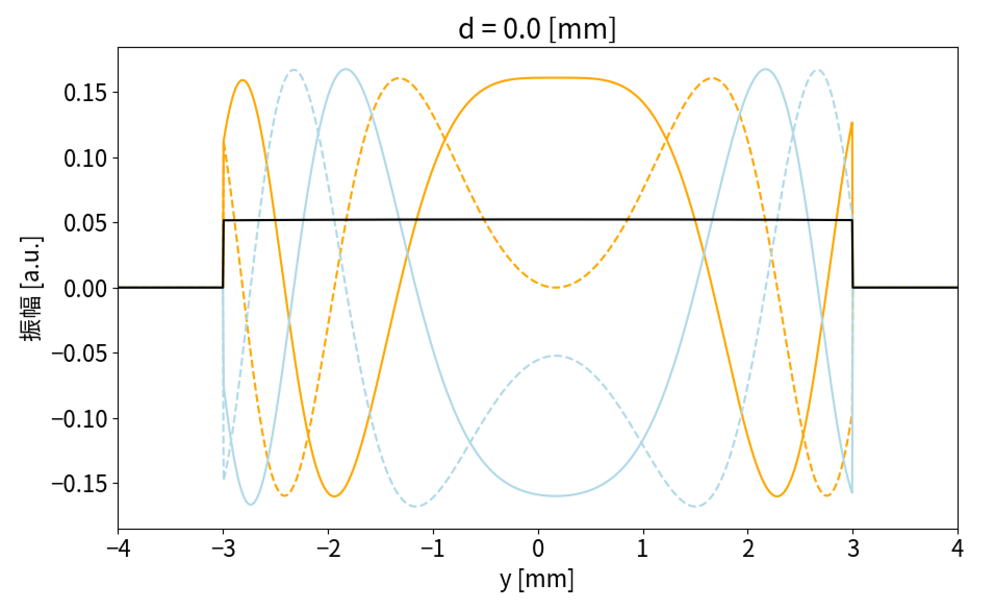
\includegraphics[width=\linewidth]{image/2-int-d00png.png}
    \subcaption{$d$ = 0 mm}
  \end{subfigure}
  \begin{subfigure}[h]{0.45\linewidth}
    \centering
    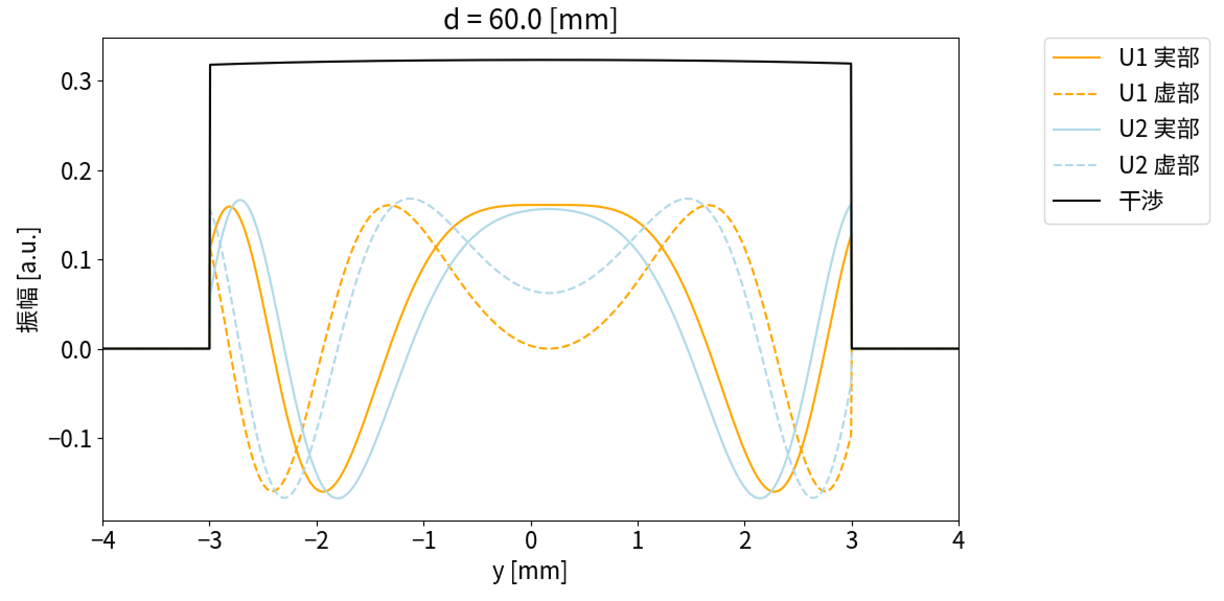
\includegraphics[width=\linewidth]{image/2-int-d60.png}
    \subcaption{$d$ = 60 mm}
  \end{subfigure}
  \caption[放射光関数の干渉項位相]{干渉項位相を導入した放射光関数。$\gamma$=380, $K$=0.971, $z$=10.26 m, $y(beam)$=0 mmのパラメータで計算した。}
  \label{fig:int}
\end{figure}

\subsection{光学関数}
光学関数は、入射光の電場振幅と位相を入力としてスクリーンにおける回折光の振幅を計算する。水平方向には平面波化されるため、回折積分は$y$軸方向のみ計算すれば十分である。
まずスリットによる入射光の遮蔽を計算する。
\begin{align}
  Slit(y) = 
  \begin{cases}
    0       &  y  < y(slit) - w(slit)\\
    Rad(y)  &  y(slit) - w(slit) \leq y \leq y(slit) + w(slit)\\
    0       &  y(slit) + w(slit) < y
  \end{cases}
\end{align}
$y(slit)$と$w(slit)$による遮蔽の計算結果の例を図\ref{fig:slit}に示す。

\begin{figure}[h]
  \begin{subfigure}[h]{0.45\linewidth}
    \centering
    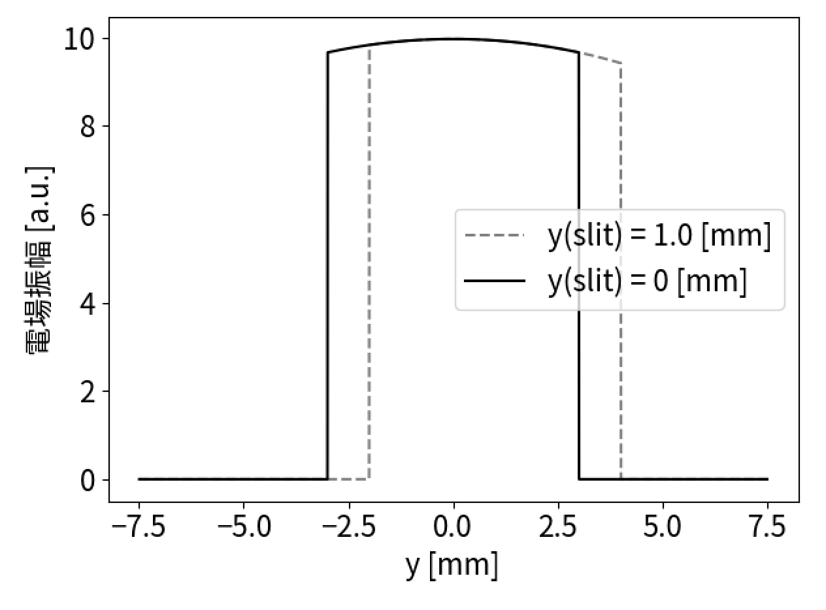
\includegraphics[width = \linewidth]{image/2-yslit.png}
    \subcaption{$y(slit)$による電場振幅の変化}
  \end{subfigure}
  \begin{subfigure}[h]{0.45\linewidth}
    \centering
    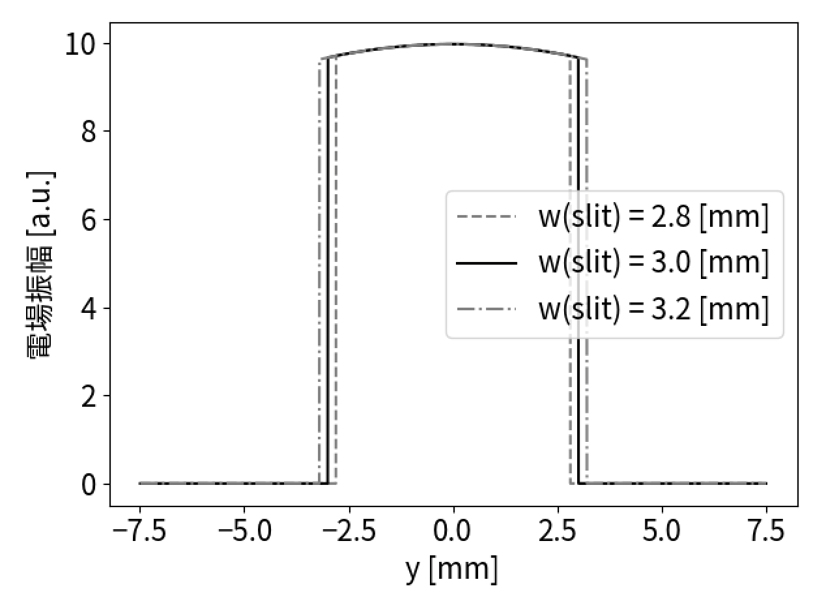
\includegraphics[width = \linewidth]{image/2-wslit.png}
    \subcaption{$w(slit)$による電場振幅の変化}
  \end{subfigure}
  \caption[光学関数のスリット座標]{パラメータ$y(slit)$と$w(slit)$。一つのアンジュレータからの放射光関数の結果を示している。
  $\gamma$=380, $K$=0.971, $z$=10.26 mのパラメータで計算した。}\label{fig:slit}
\end{figure}
次に$y$軸方向の回折をレイリー・ゾンマーフェルト積分に従って計算しカメラでの電場振幅を求め、その絶対値の二乗により規格化した光量$I(y)$が求まる。
この計算では高速フーリエ変換を用いた数値計算の高速化が可能である。詳細についてはAppendix に記述した。
\begin{align}
  I(y) = \left| \int_{slit} Slit(y')\exp(i\frac{2\pi}{\lambda_L} \sqrt{z(slit-cam)^2 + (y-y')^2})\text{d}y' \right|^2 
\end{align}
この時$z(slit-cam)$が回折計算のパラメータとなる(図\ref{zp})。
\begin{figure}[H]
  \centering
  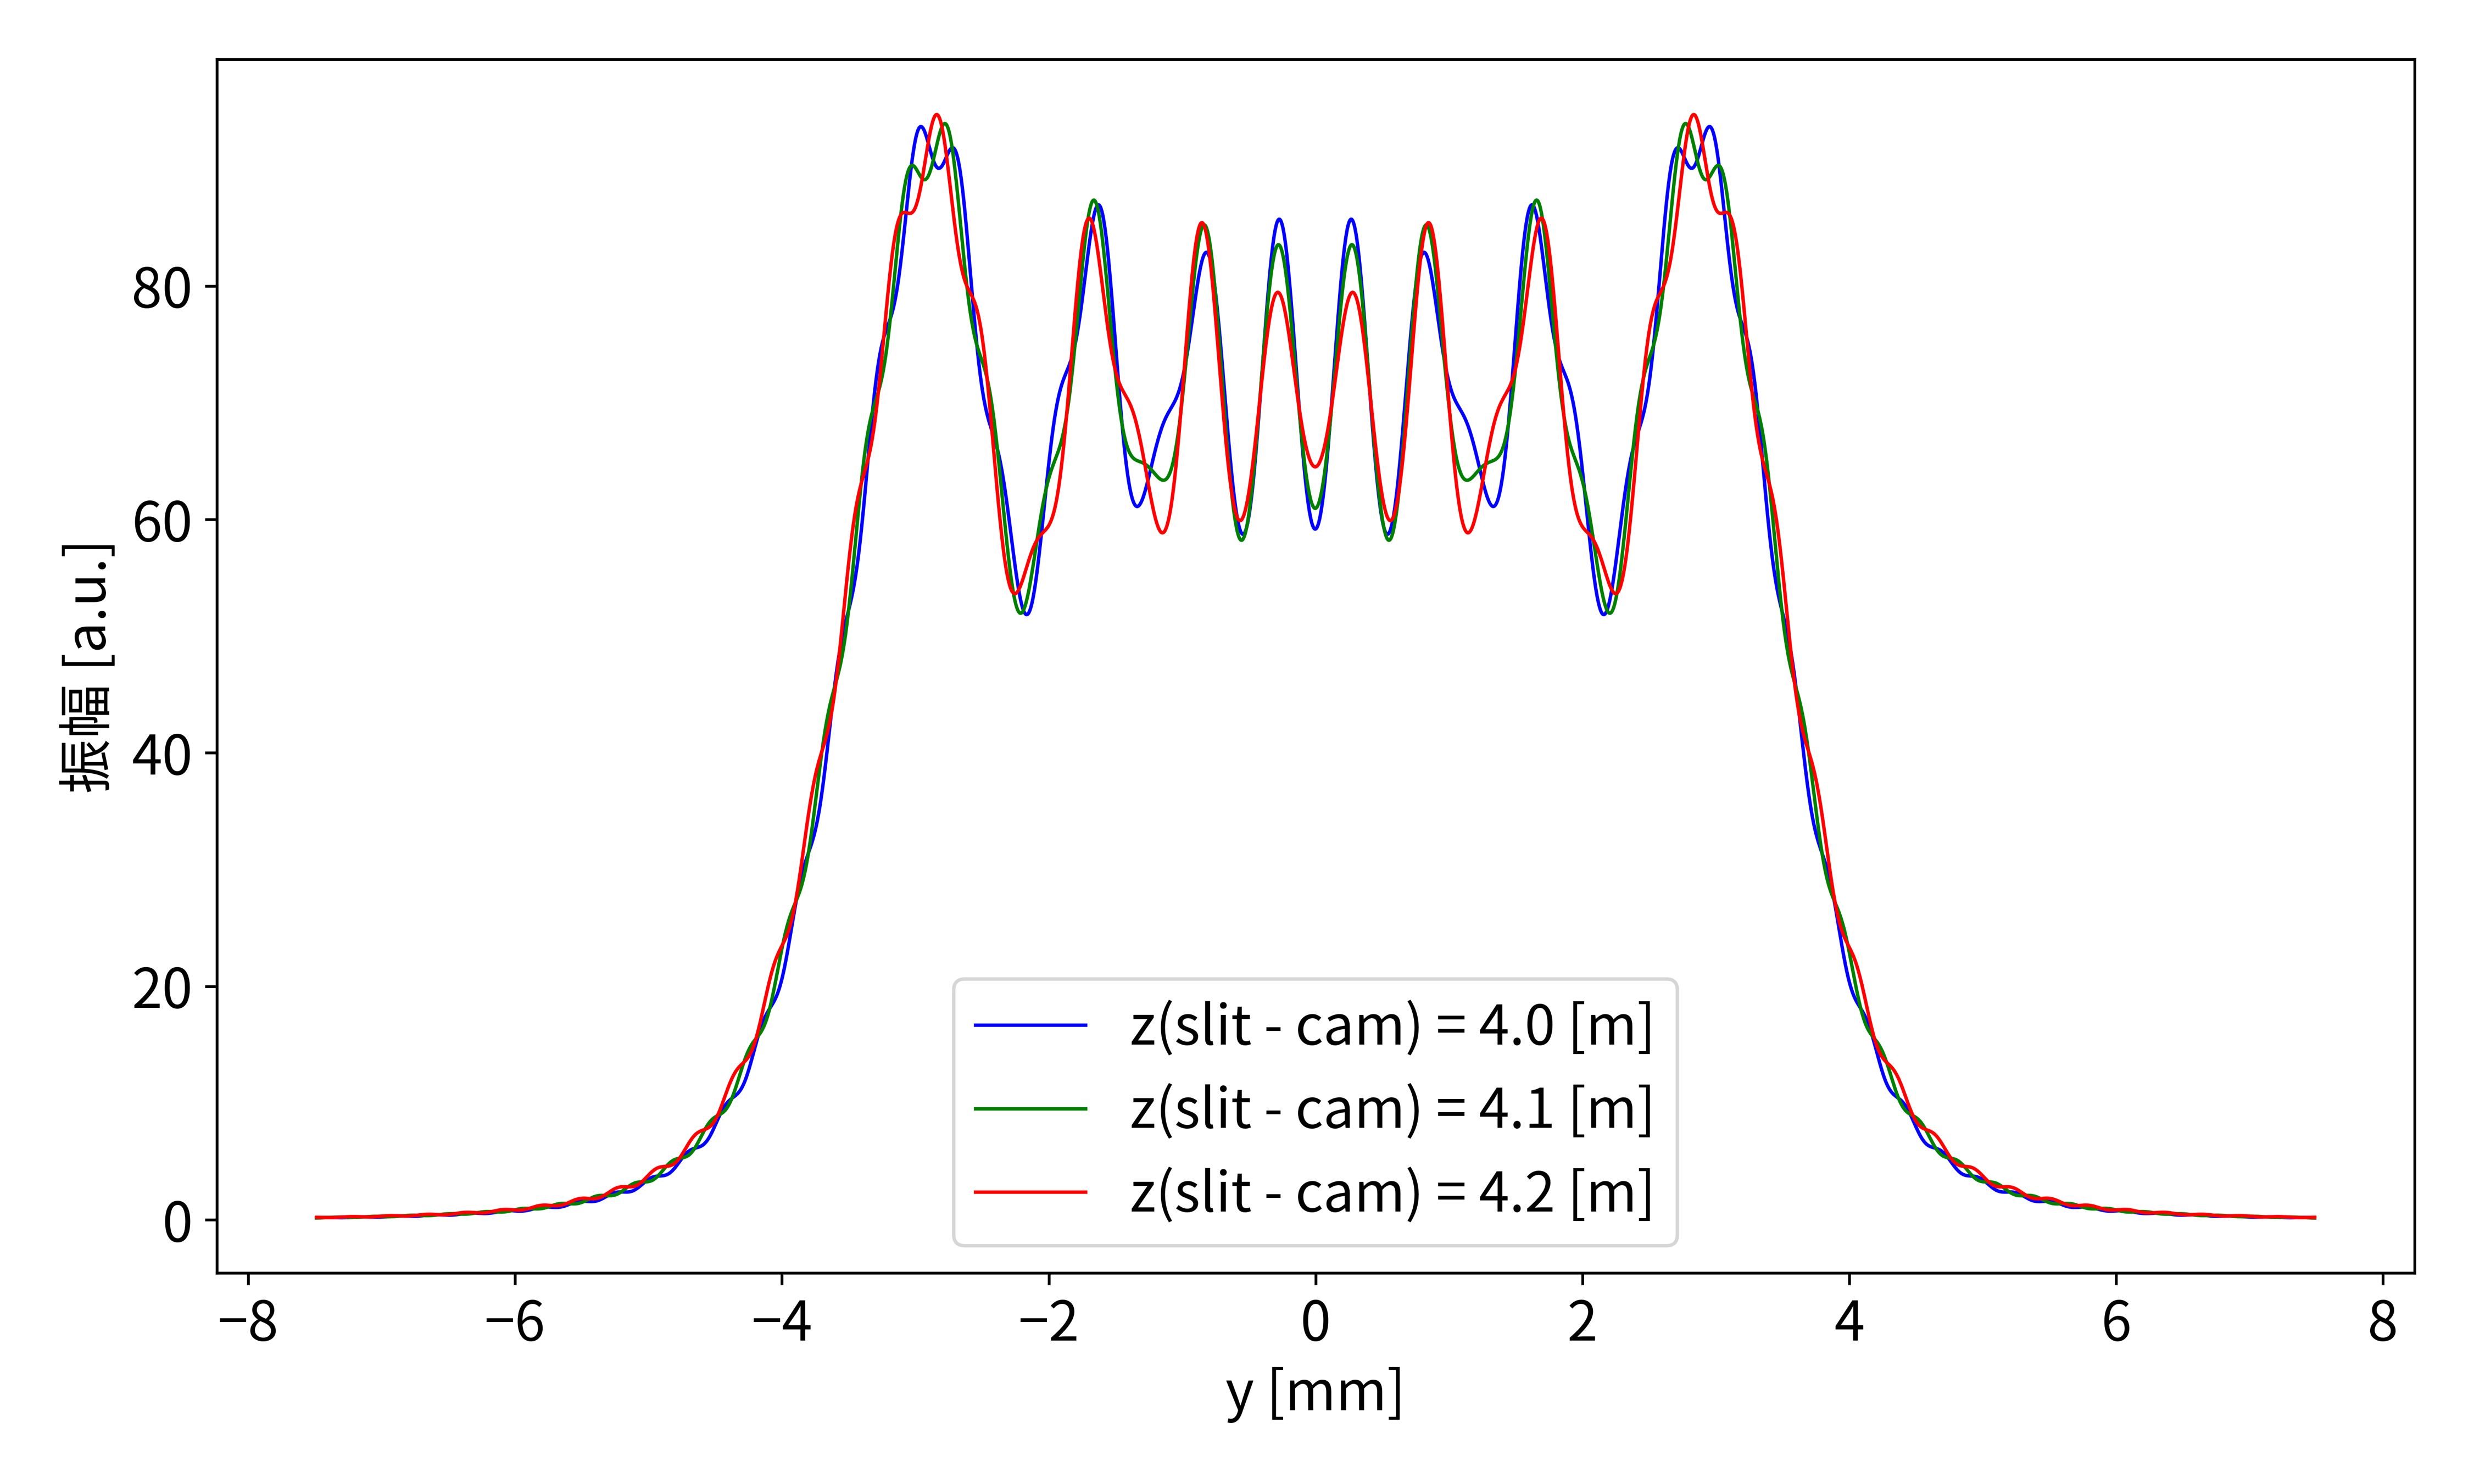
\includegraphics[width = 0.8\linewidth]{image/2-zp.png}
  \caption[光学関数のスリット-カメラ間距離]{光学関数の計算におけるパラメータ$z(slit-cam)$依存性。$\gamma$=380, $K$=0.971, $z$=10.26 mのパラメータで計算した。}\label{zp}
\end{figure}

ここまでの計算によって、モデル関数の$y$依存性が放射光および光学の物理モデルによって再現でき、規格化された光量の分布が得られる。
最後に振幅の比例係数$ampl$を導入することで、実際の光量に合わせたモデル関数を得ることができる。
\begin{align}
  Model(y|\lambda_L,d) = ampl \times I(y) 
\end{align}
原則として、全ての$d$に対して共通のパラメータの組を用いてモデル関数によるフィットを行う。

\section{単独アンジュレータの解析}
\noindent \textbf{\underline{解析}}\par
$ampl$パラメータ較正を目的として、単独アンジュレータのデータを解析した。
下流アンジュレータのみによって得られるデータから、放射光関数の$d$依存性の情報が抽出できる。
理想的な条件では、アンジュレータが下流に移動すると以下のような変化が見られると考えられる。
\begin{itemize}
  \item アクセプタンスの増加による振幅の増加
  \item 光学的な位置関係の変化による回折パターンの形状の変化
\end{itemize}

振幅の上昇と回折パターンの形状の変化から、放射光の光量に対応する振幅係数がアンジュレータの位置に対してどのように依存するかを解析する。
カメラで撮影された画像は回折像であるから、隣り合うピクセル同士の(回折の効果がなかった時の)真のピクセル値が互いに相関している。
そのため、あるピクセルに注目しその$d$依存性を調べるだけでは十分な情報が得られないことが期待される。
したがって、回折の効果を取り入れたフィッティングによって、ある位置での回折像全体($I(y|d)$)にかかる係数$ampl(d)$を求めることが有効であると考えた。
%距離のパラメータ $z(U2-slit),z(slit-cam),w(slits)$の最適値を求めることができる。
%$z(U2-slit),z(slit-cam),w(slit)$を固定してフィッティングを行い、適合度がもっとも良いパラメータの組を最適な値として定義する。
上流アンジュレータに関するパラメータを除いたパラメータをフィットに用いた(表\ref{tab:single_prm})。

  

\noindent \textbf{\underline{結果}}\par
電子ビームエネルギー210 MeVにおいて取得した単独アンジュレータのデータを解析した。
モデル関数のうち、下流アンジュレータの放射光関数と光学関数のみを用いて回折パターンを計算し、
既約カイ二乗を用いた最小二乗法でフィットを行う。また、フィットにはpythonのiminuitモジュール\cite{iminuit}を用いた。
%\subsubsection{波長依存性}
%波長依存性があり長波長側の光量が大きい傾向がある。
%この傾向は線形の依存性が仮定できる。\\
\subsubsection{位置依存性}
アンジュレータが下流に移動することによる回折パターンの変化を図\ref{DCposdep}に示す。上流側のパターンと比較すると、下流側($d= 825$)の回折パターンは振幅が大きくなり、回折パターン全体の幅が広がっていることがわかる。
また回折パターンは上流下流にかかわらず8つのピークがあるが、ピーク同士の相対的な高さの変化も見られる。
\begin{figure}[H]
  \centering
  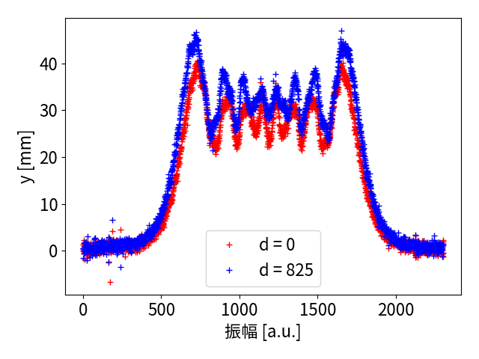
\includegraphics[width=0.8\linewidth]{image/4-DCposdep.png}
  \caption[アンジュレータ位置依存性]{単独アンジュレータデータの位置依存性。アンジュレータが最上流(赤)と最下流(青)に移動したときの回折パターンを比較すると、振幅やパターン全体の幅、回折のピーク同士の高さが変化していることがわかる。}\label{DCposdep}
\end{figure}

回折パターンの形状の変化はモデル関数において、放射光関数の球面波位相が変化することで説明できると考えられる。
振幅の変化は、$ampl$パラメータを$d$によって変化するパラメータ$ampl(d)$としてフィッティングを行うことで詳しく調べられる。
また、単独アンジュレータの画像では上流と下流のアンジュレータ放射の干渉がなく、波長によって回折画像がほとんど変わらないと考えられるから、波長方向にピクセルの平滑化を行った。
500~ピクセルの平滑化を行ったデータに対するフィットの結果を図\ref{single_d}に示した。平滑化によって回折パターンの微細構造が見えており、フィット結果がこの構造を再現していることがわかる。
この時のフィット結果を表\ref{tab:single_prm}に示した。

また、平滑化を行わないデータを用いてフィットを行った結果、$\chi^2/\text{ndf} = 1.56$となった。
一方500~ピクセルの平滑化を行い、ピクセル値の誤差を500~ピクセル$\times$4枚の画像の計2000~ピクセルの標準誤差を誤差としてフィットを行った結果、
$\chi^2/\text{ndf} = 13.0$となり、誤差を過小評価している可能性がある。

\begin{figure}[H]
  \centering
  \begin{subfigure}[h]{0.45\linewidth}
    \centering
    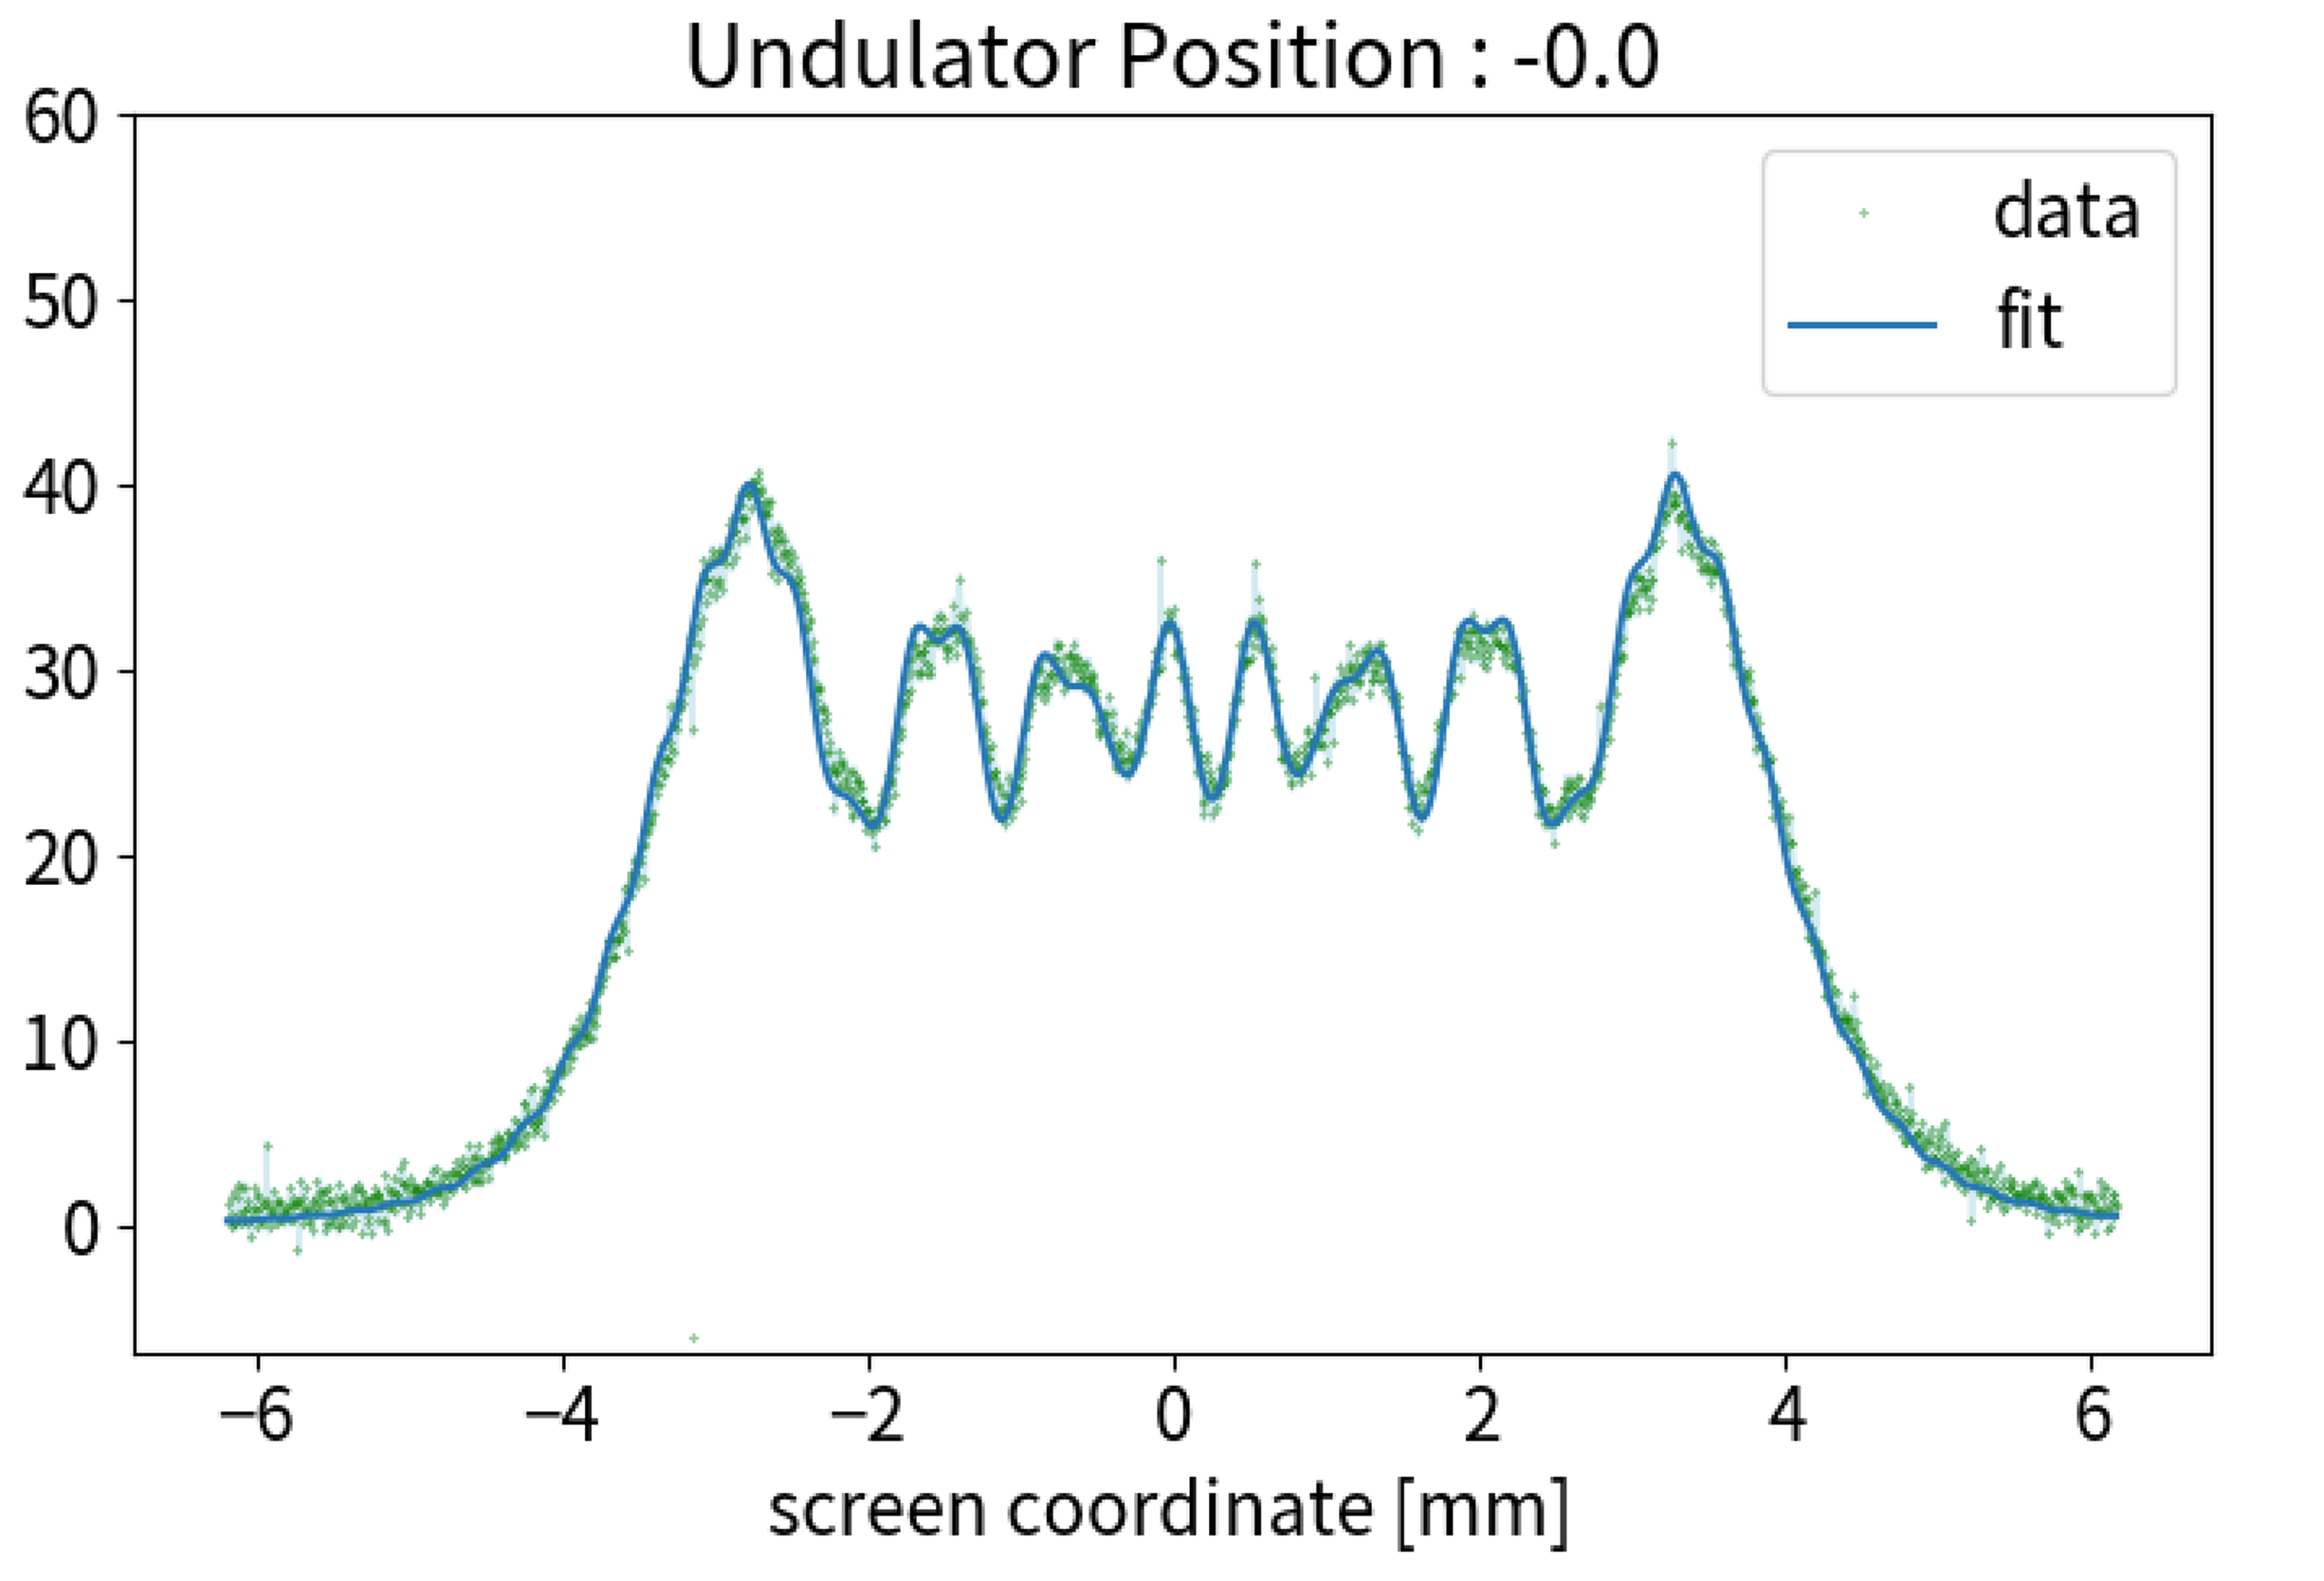
\includegraphics[width=\linewidth]{image/4-single_0.png}
    \subcaption{$d$=0~mm}
  \end{subfigure}
  \hfill
  \begin{subfigure}[h]{0.45\linewidth}
    \centering
    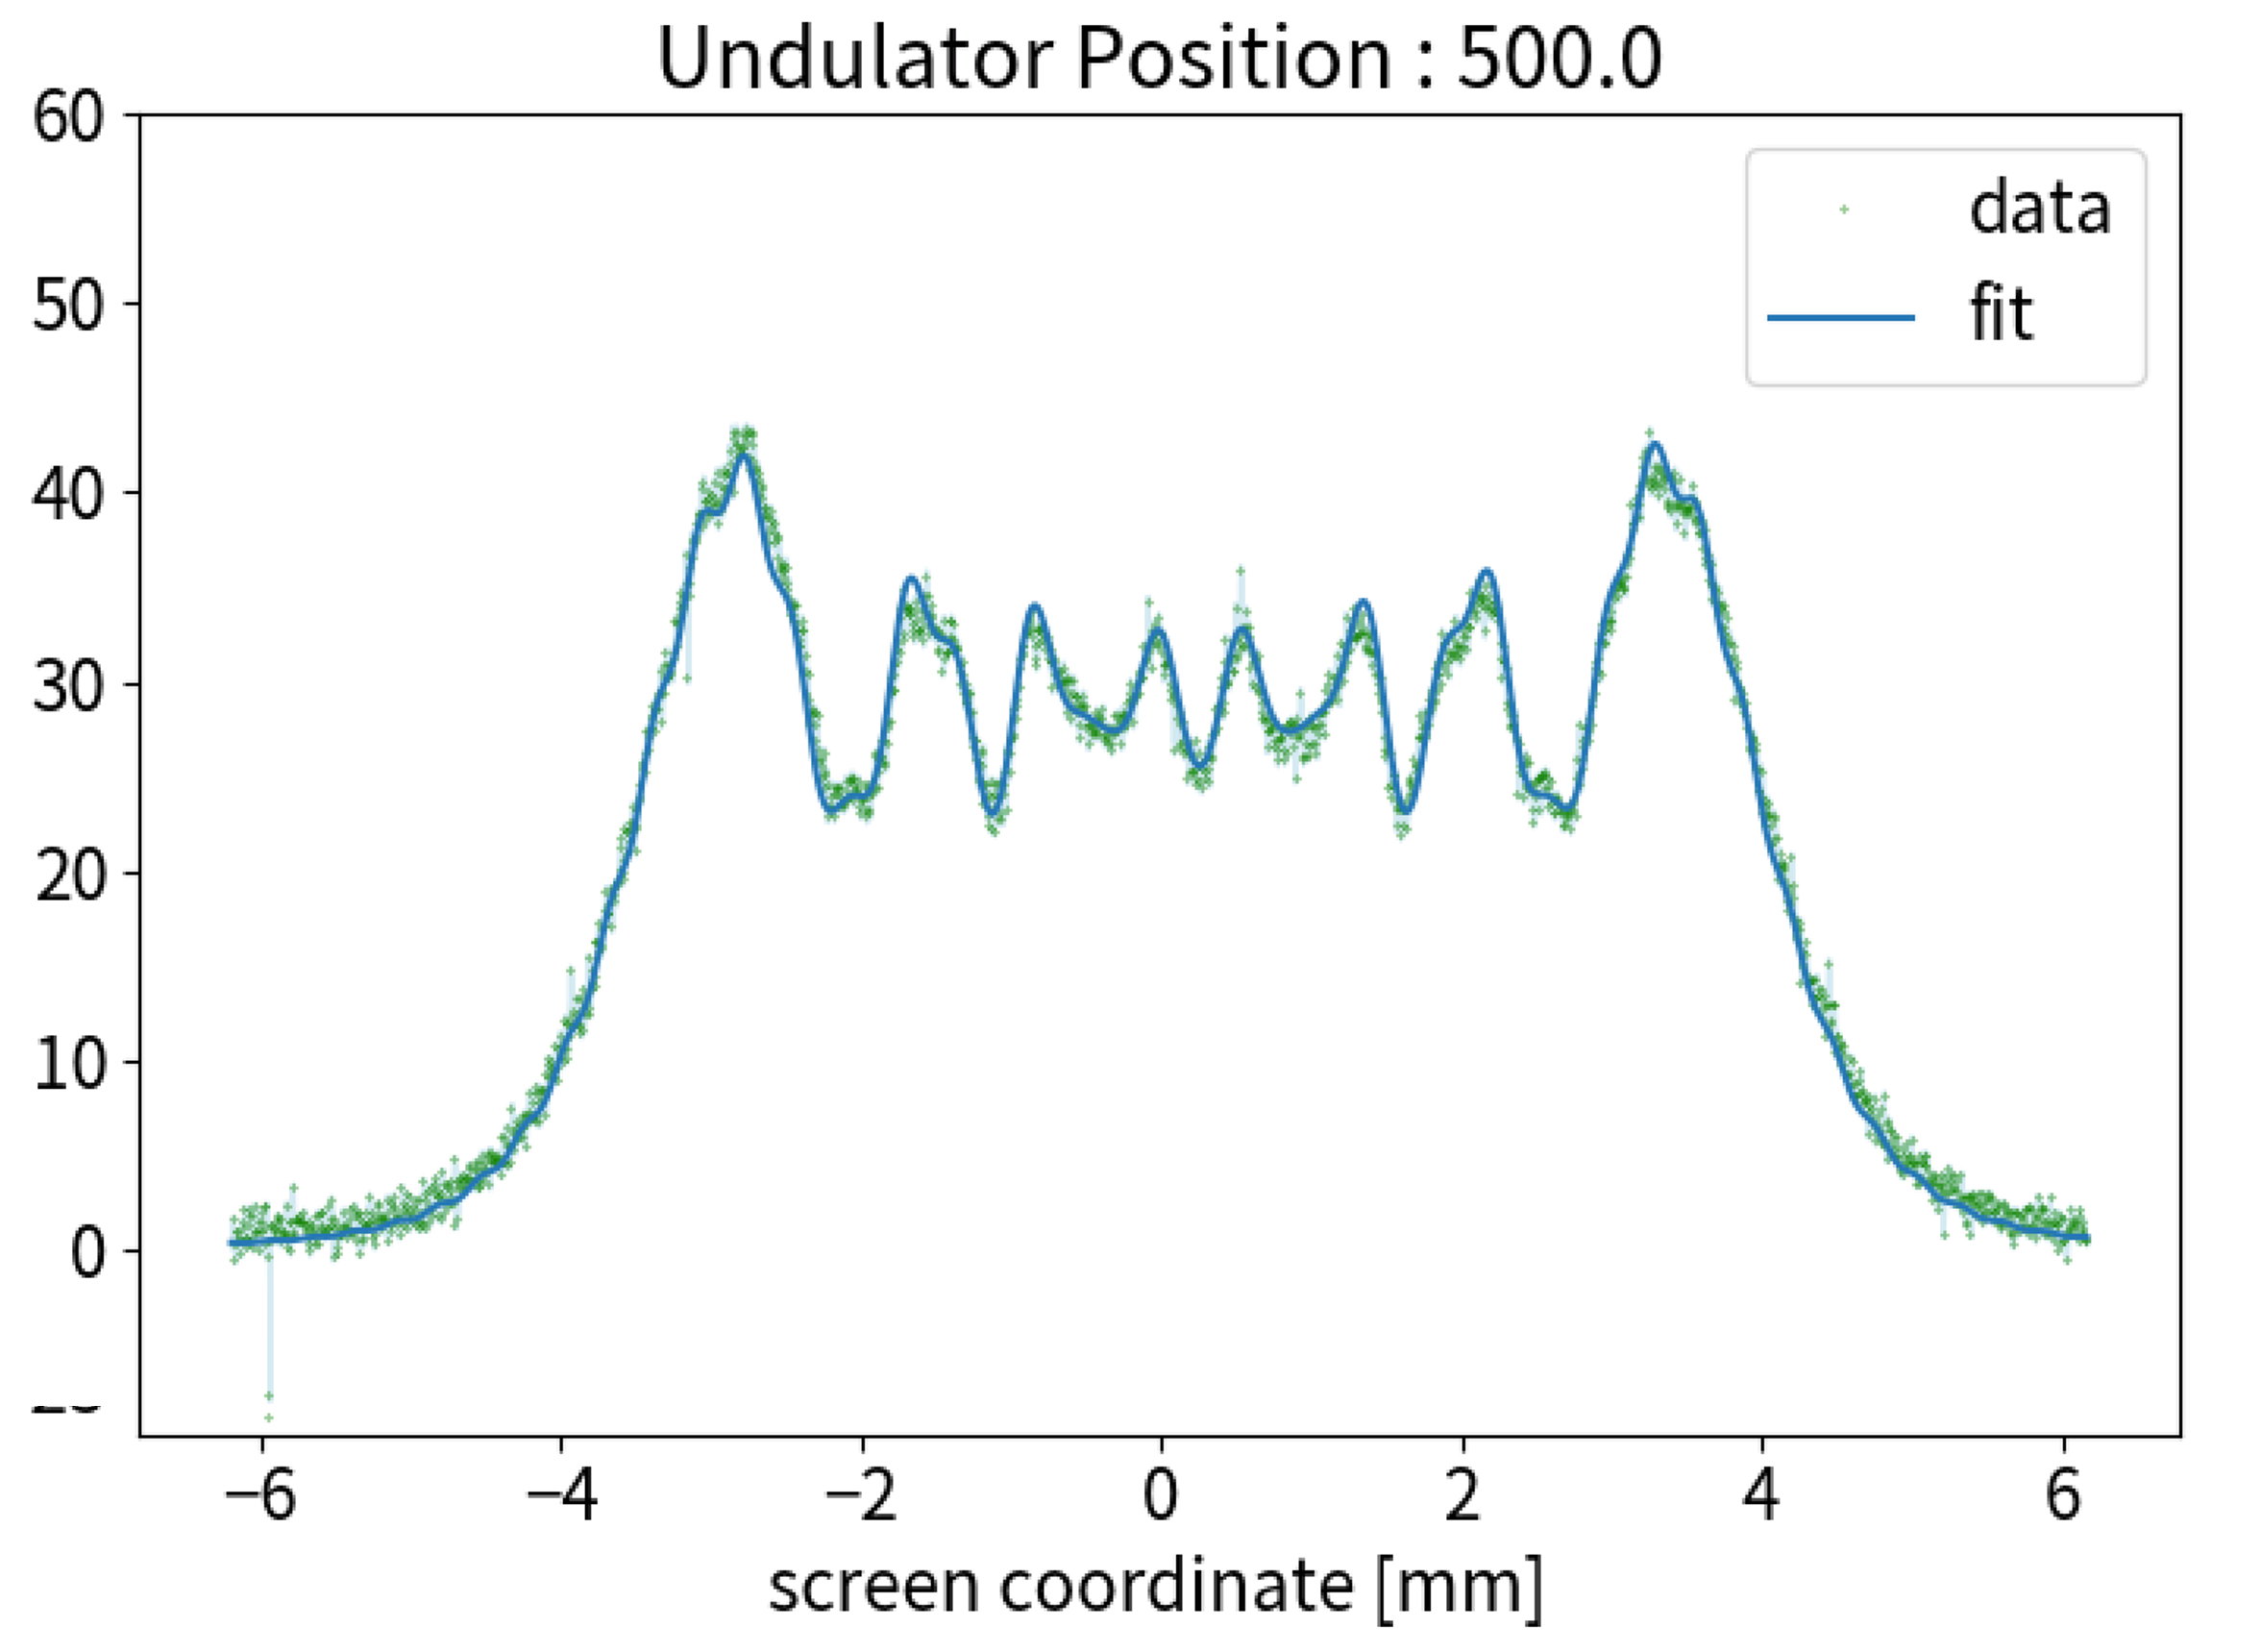
\includegraphics[width=\linewidth]{image/4-single_500.png}
    \subcaption{$d$=500~mm}
  \end{subfigure}
  \caption[単独アンジュレータのデータ]{単独アンジュレータでの回折像のフィッティング結果を示す。波長方向(画像の$x$軸方向)に500ピクセルの平滑化を行ったため、
  明瞭な回折パターンが見られる。フィットの結果はこのパターンをよく再現している。}\label{single_d}
\end{figure}

\begin{table}
  \centering
  \begin{tabular}{c|c|cc}
    パラメータ & 初期値 & 最適値 & 誤差(ヘッシアン誤差)\\ \hline
    $\gamma$  & 410        & 407.16 & 0.13\\
    $\sigma_y$ & 50~$\mu$m & 51.9~$\mu$m& 0.5~$\mu$m\\
    $z(U2-slit)$ & 10.26~m & 10.015~m & 0.027~m\\
    $z(slit-cam)$ & 4.11~m & 4.169~m & 0.004~m\\
    $w(slit)$ & 3~mm       & 3.070~mm& 0.002~mm\\
    $y(beam)$ & 0.25~mm    & 0.22~mm& 0.01~mm\\
    $y(slit)$ & 0.25~mm    & 0.248~mm&0.03~mm \\
    $ampl$ & -             &図\ref{DCampl}&-\\
  \end{tabular}
  \caption[単独アンジュレータのフィッティングパラメータ]{単独アンジュレータのフィッティングパラメータ。210 MeVにおいては共鳴波長から外れた波長で観測を行っているため、
  放射光の電場振幅の概形が$\gamma$に大きく依存する。そのため$\gamma$を自由なパラメータとして扱いフィットを行った。$ampl$パラメータは後述のとおり、$d$に依存するパラメータとして導入する} 
  \label{tab:single_prm}
\end{table}

フィッティングの結果得られた$ampl$パラメータを$d$に対してプロットした結果を図\ref{DCampl}に示す。
$d$に対して全体的に上昇する傾向と、周期的に変動する傾向が見られる。この周期的変動は約135~mmであり、
測定に用いた電子ビームエネルギー210 MeVに対応する周期的変動の周期(式(\ref{zero order energy formula}))$\lambda_{osc} = 2\gamma^2\lambda_L \simeq 135~\text{mm}$に一致している。
これはアンジュレータ放射光と可干渉で、$d$に依存しない位相の光波が入射しており、この光波と下流アンジュレータの放射光の
相対的な位相が$d$に依存して変化していると考えられる。偏向電磁石によるシンクロトロン放射はこの条件を満たしており、
アンジュレータ下流の偏向電磁石による放射が単独アンジュレータの放射光の観測では無視できないと結論付けられる。

また、振幅の上昇が、アクセプタンスの増加によるものだと仮定すると、振幅は見込む立体角に比例すると近似できるから、
$d$依存性は$1/z(U2-slit)^2$を反映したものになると考えられる。これらの仮定を踏まえて
\begin{eqnarray}
  ampl(d) = \frac{1}{(z(U2-slit) -d)^2} + \sin\left( \frac{2\pi}{\lambda'_{osc}}d + \phi \right)\label{eq:ampl}
\end{eqnarray}
というモデル関数を用いてフィッティングを行うと、$z(U2-slit) = 10.51$ m、$\lambda'_{osc}= 135.33$ mmという値が得られた。
実測値$z(U2-slit)$ = 10.26~mに対して0.25~mのずれがある。この値はアンジュレータの中心とスリットまでの実測値であり、アンジュレータの長さ$0.52$~mを考慮すると
アンジュレータの最上流からスリットまでの距離よりも短い。そのためこのずれはアンジュレータの長さの効果を取り入れた実効的な距離として解釈できる。
また、アンジュレータの長さやビームサイズの効果によって実効的な距離の変化が生じることが考えられる。

\begin{figure}[h]
  \centering
  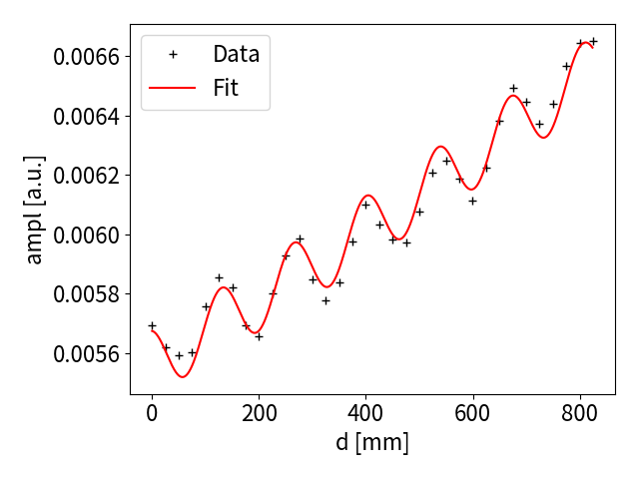
\includegraphics[width=0.8\linewidth]{image/4-DCampl.png}
  \caption[アンジュレータ位置依存性]{アンジュレータ位置に対する$ampl$パラメータの変化。アンジュレータが下流(d =825 側)に移動すると振幅が増加すると
  ともにおよそ135~mm周期で振動する傾向が見られる。}\label{DCampl}
\end{figure}

この結果から光量が距離の二乗に反比例することを確認できた。2台のアンジュレータで用いる$ampl$パラメータの関係を
\begin{align}
  ampl(d) &= \frac{ampl}{z(U-slit)^2}\label{eq:ampl_dep}\\
   z(U-slit) & = 
  \begin{cases}
     z(U1-slit)\\
     z(U2-slit) - d
  \end{cases}
\end{align}
の式に従って定義することができる。
これにより、2台のアンジュレータの解析では一つの$ampl$パラメータを用いて、位置による光量の変化を式(\ref{eq:ampl_dep})によって表現することができる。

一方、フィットによって得られた$z(U2-slit)$パラメータの値は10.015 mであり、振幅の増加に対する$ampl(d)$のフィットの結果が実測値よりも長くなったこととは逆の結果を示している。
しかしモデル関数内の$z(U2-slit)$パラメータは主に放射光関数の球面波位相を決定するパラメータであり、位相に対する実効的な距離パラメータは
光量の増加に対する実効的な距離パラメータと独立であると考えても矛盾しない。
また、$z(U2-slit)$パラメータの値は球面波位相の仮定のもとでの最適値であることや、$z(slit-cam)$パラメータや$w(slit)$パラメータと相関することが考えられるため
単独アンジュレータの解析によって得られた$z(U2-slit)$パラメータは2台のアンジュレータの解析には用いないこととする。

$\gamma$パラメータは、本来のエネルギーの値210 MeVに対応するおよそ$\gamma =410$と比較すると$\gamma = 407$であり小さい。
$\gamma$は放射光関数の電場振幅に大きな寄与を与えており、$\gamma$が小さいことは放射光関数の関数形が実際の放射光関数と異なることを示唆している。


\section{2台のアンジュレータの解析}
\noindent \textbf{\underline{解析}}\par
上流のアンジュレータの放射光関数と干渉項を加えた完全なモデル関数を用いて解析する。
動かすパラメータを表\ref{tab:double}に示した。
フィッティングは既約カイ二乗による最小二乗法を用いる。
またpythonのlmfitパッケージ\cite{lmfit}を用いてフィッティングを行う。
iminuitと比較して単純化されたフィットルーチンのため、複雑なパターン構造のデータに対しても少ない試行回数で高速にフィットすることができる\\
フィットによって得られた$\gamma$の最適値から電子ビームを求める。

\noindent \textbf{\underline{結果}}\par
図\ref{images}に2台のアンジュレータで得られる画像の例を示す。アンジュレータの位置$d$によって回折パターンの形状が変化することがわかる。波長によって振動の初期位相が違うため、強弱が長波長側に移動していくように見える。
\begin{figure}[H]
  \centering
  \includegraphics[width=0.8\linewidth]{image/4-images.png}
  \caption[干渉による画像の変化]{2台のアンジュレータで得られた画像の変化}\label{images}
\end{figure}

較正波長404.65 nm、$y = 0$のピクセルの周期的変動を、アンジュレータの位置$d$に対してプロットした結果の例を示す。周期的変動がみられることがわかる。
\begin{figure}[H]
  \centering
  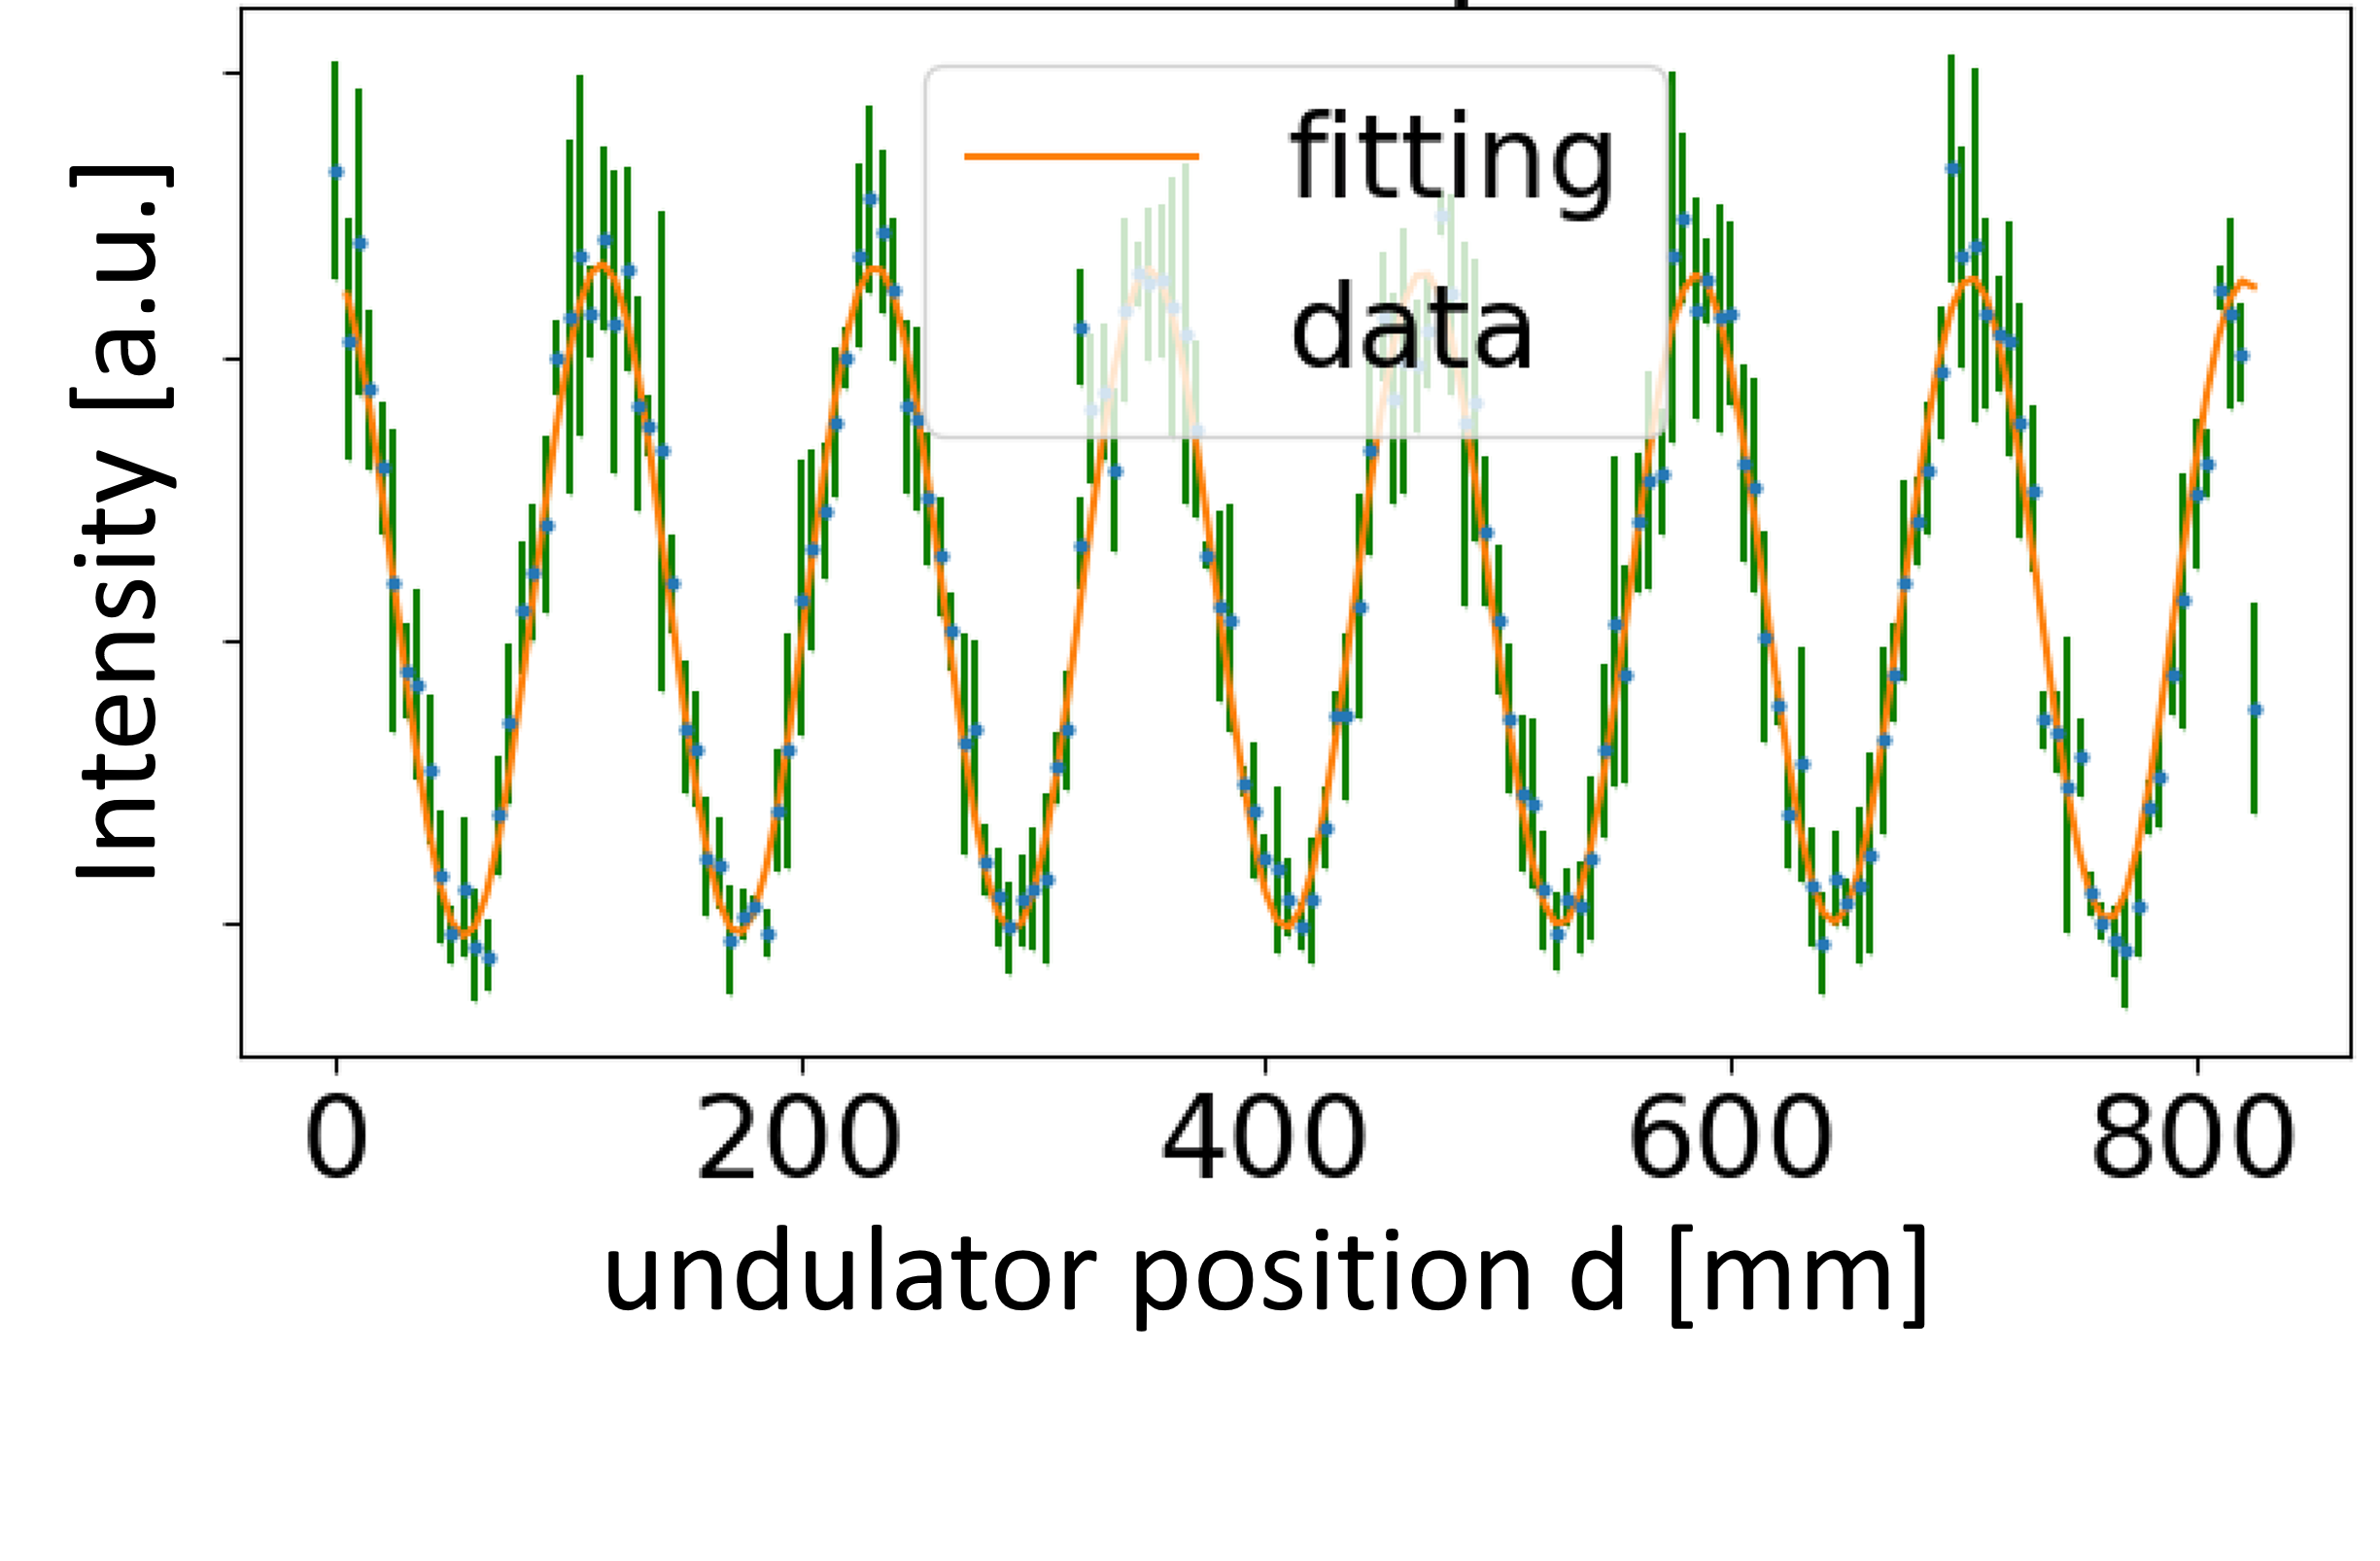
\includegraphics[width=0.8\linewidth]{image/4-oscillation.png}
  \caption[アンジュレータ位置に対する振幅の変化]{アンジュレータ位置に対する振幅の変化。較正波長 404.65 nm、$y$ =0 mmのピクセルを選び、ピクセル値を$d$に対してプロットすると周期的変動が見られる。}
\end{figure}
%fittingの結果
この画像をフィッティングした結果を図\ref{fig:double}に示す。周期的な振動と、回折パターンの両方がフィットできている。またフィットしたパラメータの結果を表\ref{tab:double}に示す。
\begin{figure}[H]
  \centering
  \begin{subfigure}[h]{0.45\linewidth}
    \centering
    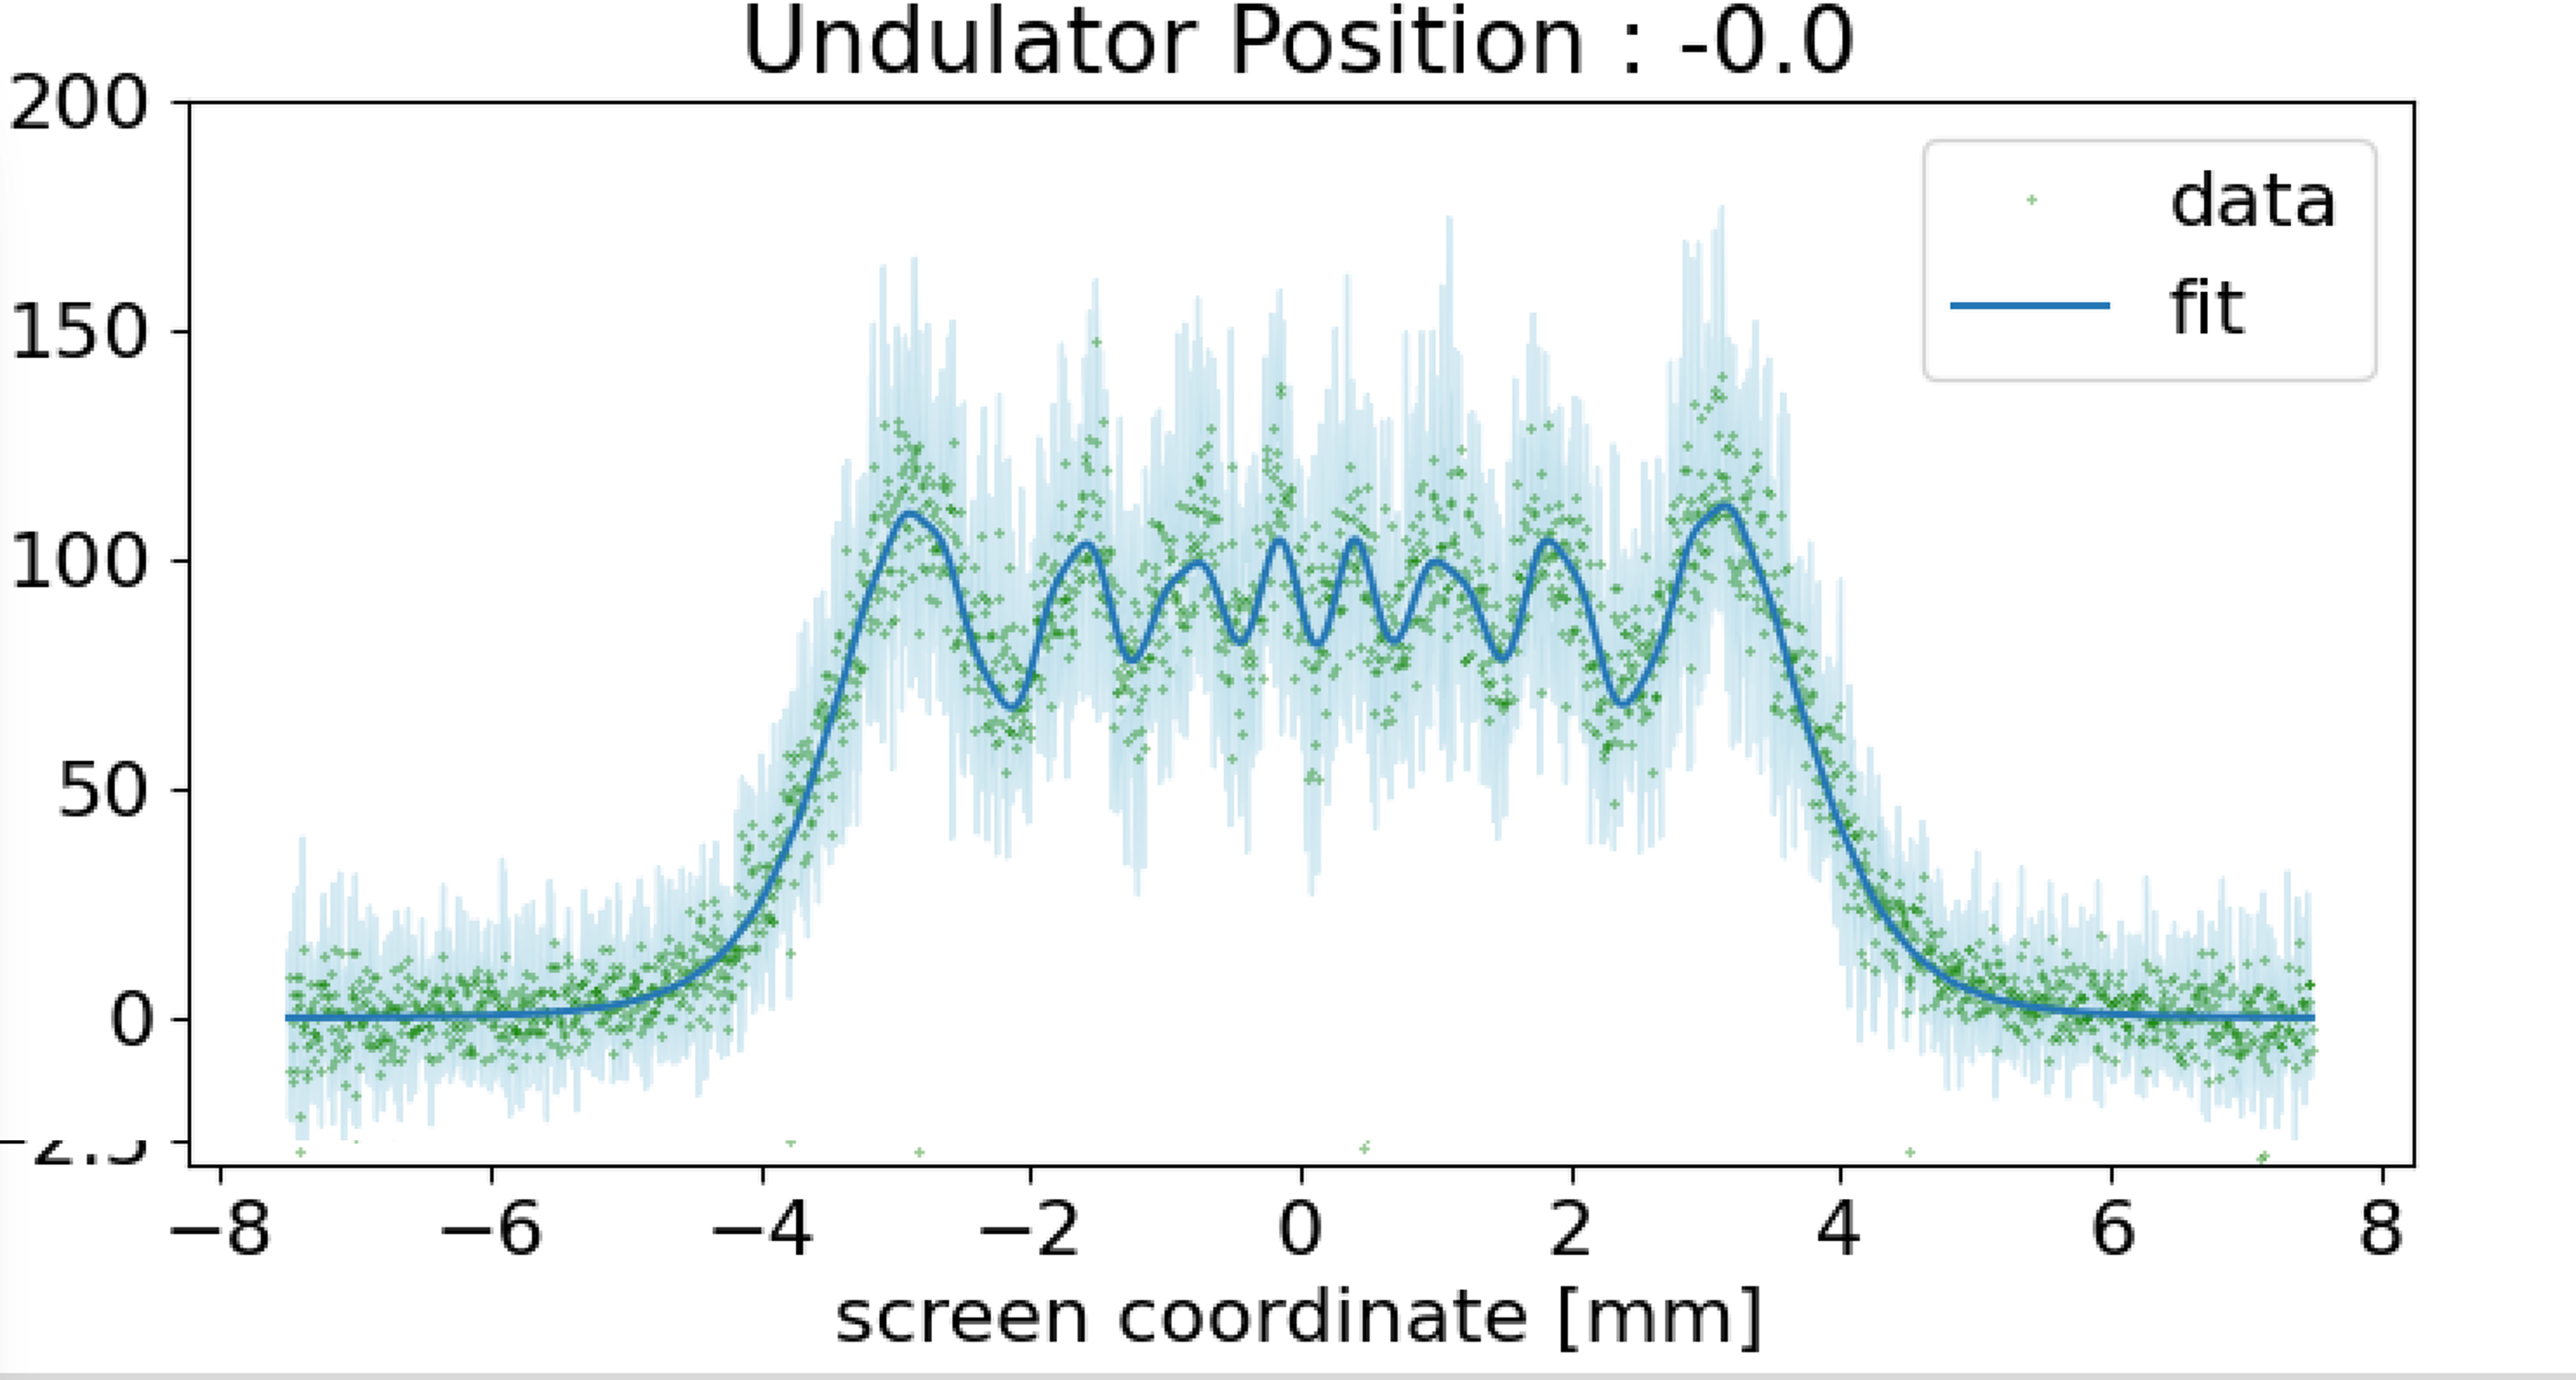
\includegraphics[width=\linewidth]{image/4-double_0.png}
    \subcaption{$d$=0~mm}
  \end{subfigure}
  \hfill
  \begin{subfigure}[h]{0.45\linewidth}
    \centering
    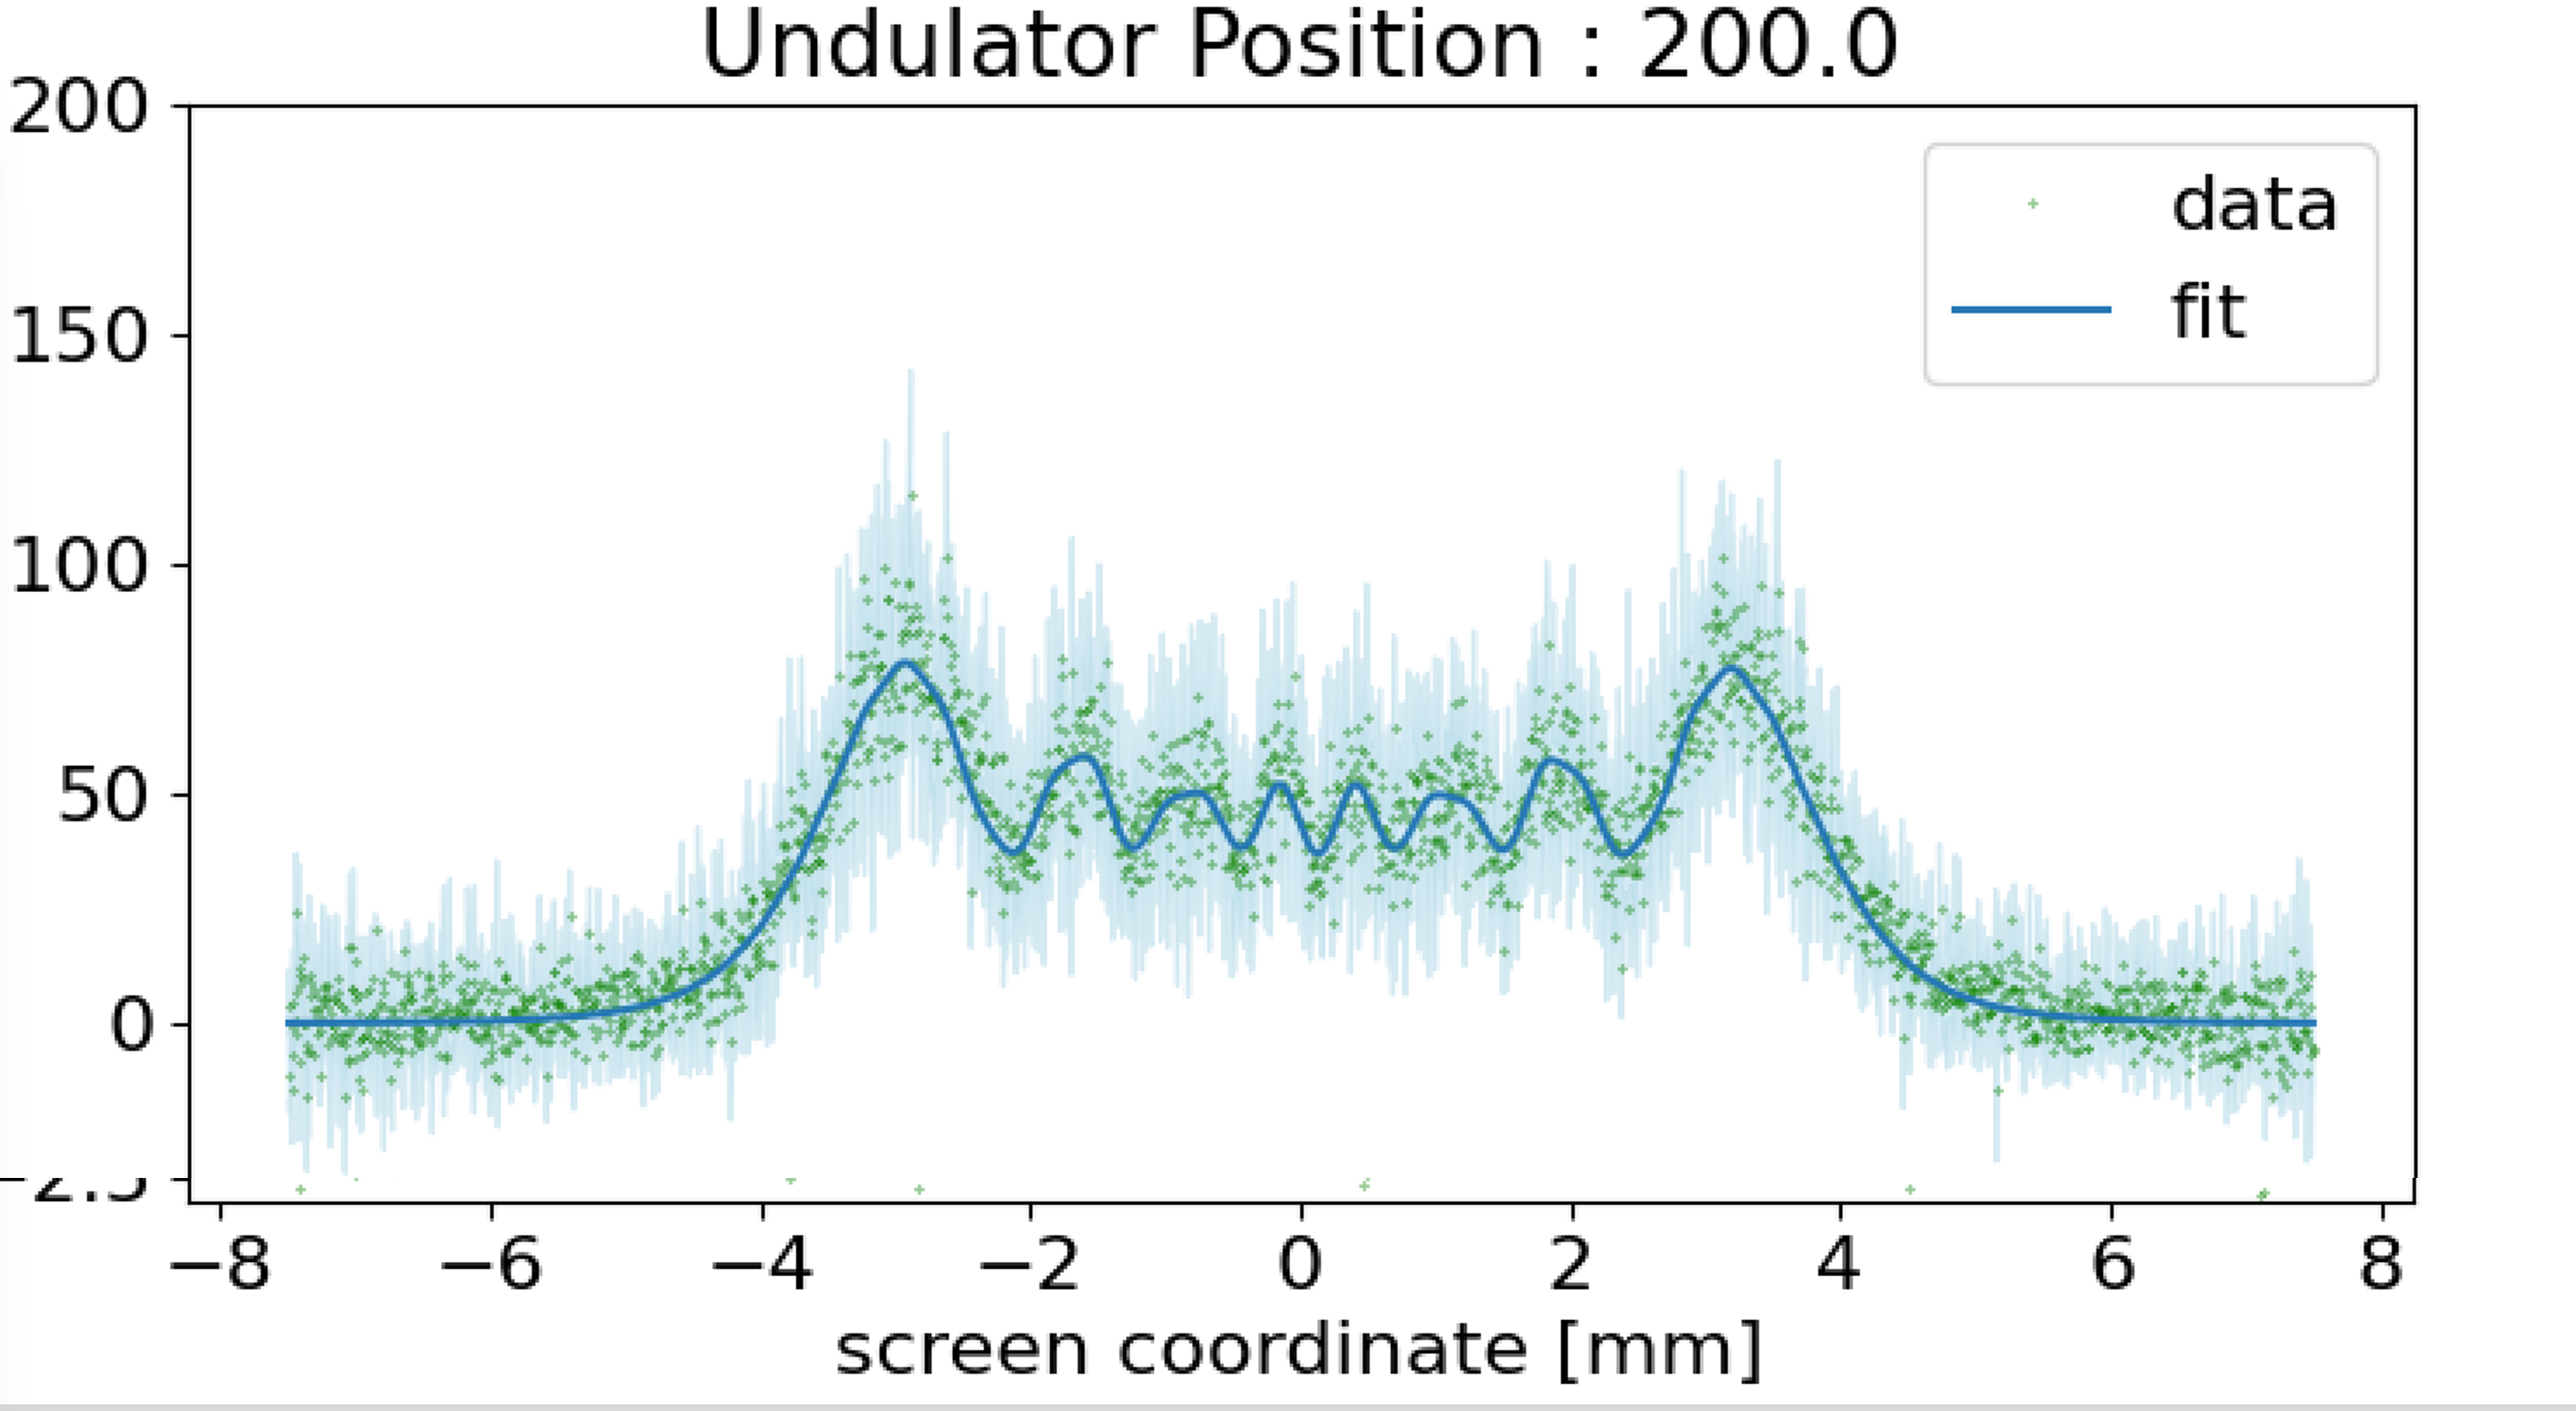
\includegraphics[width=\linewidth]{image/4-double_200.png}
    \subcaption{$d$=200~mm}
  \end{subfigure}
  \begin{subfigure}[h]{0.45\linewidth}
    \centering
    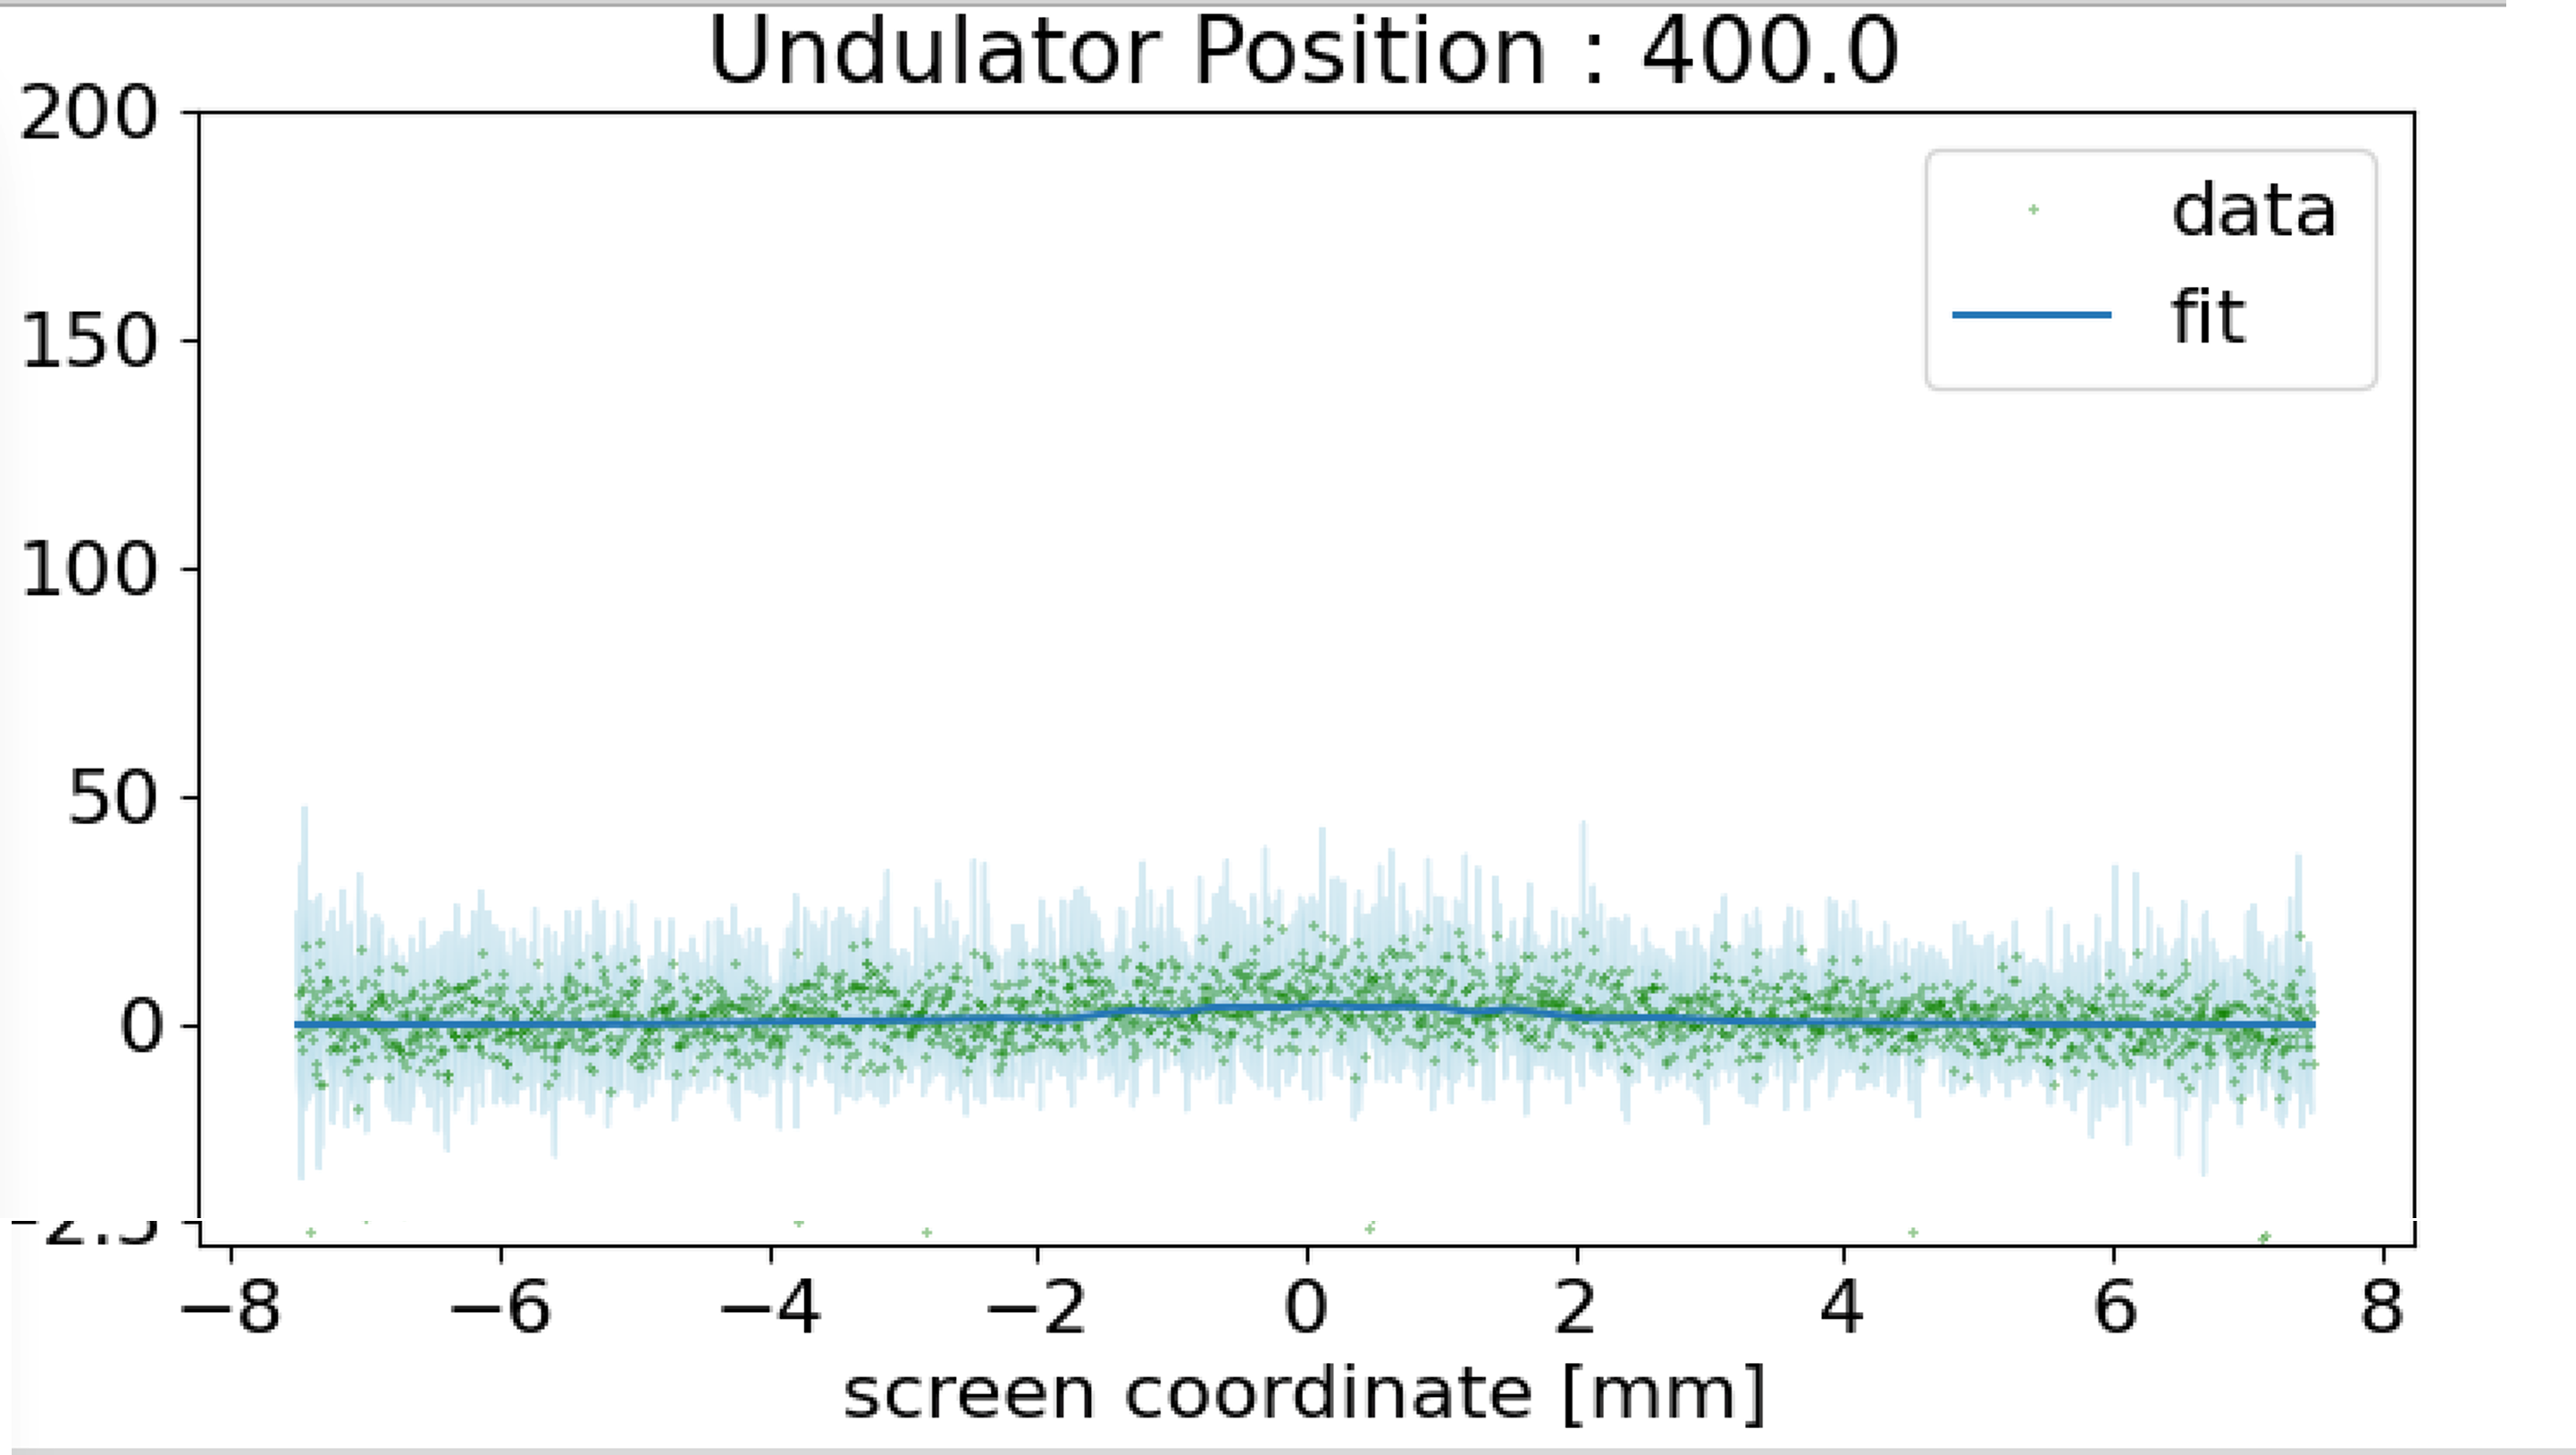
\includegraphics[width=\linewidth]{image/4-double_400.png}
    \subcaption{$d$=400~mm}
  \end{subfigure}
  \hfill
  \begin{subfigure}[h]{0.45\linewidth}
    \centering
    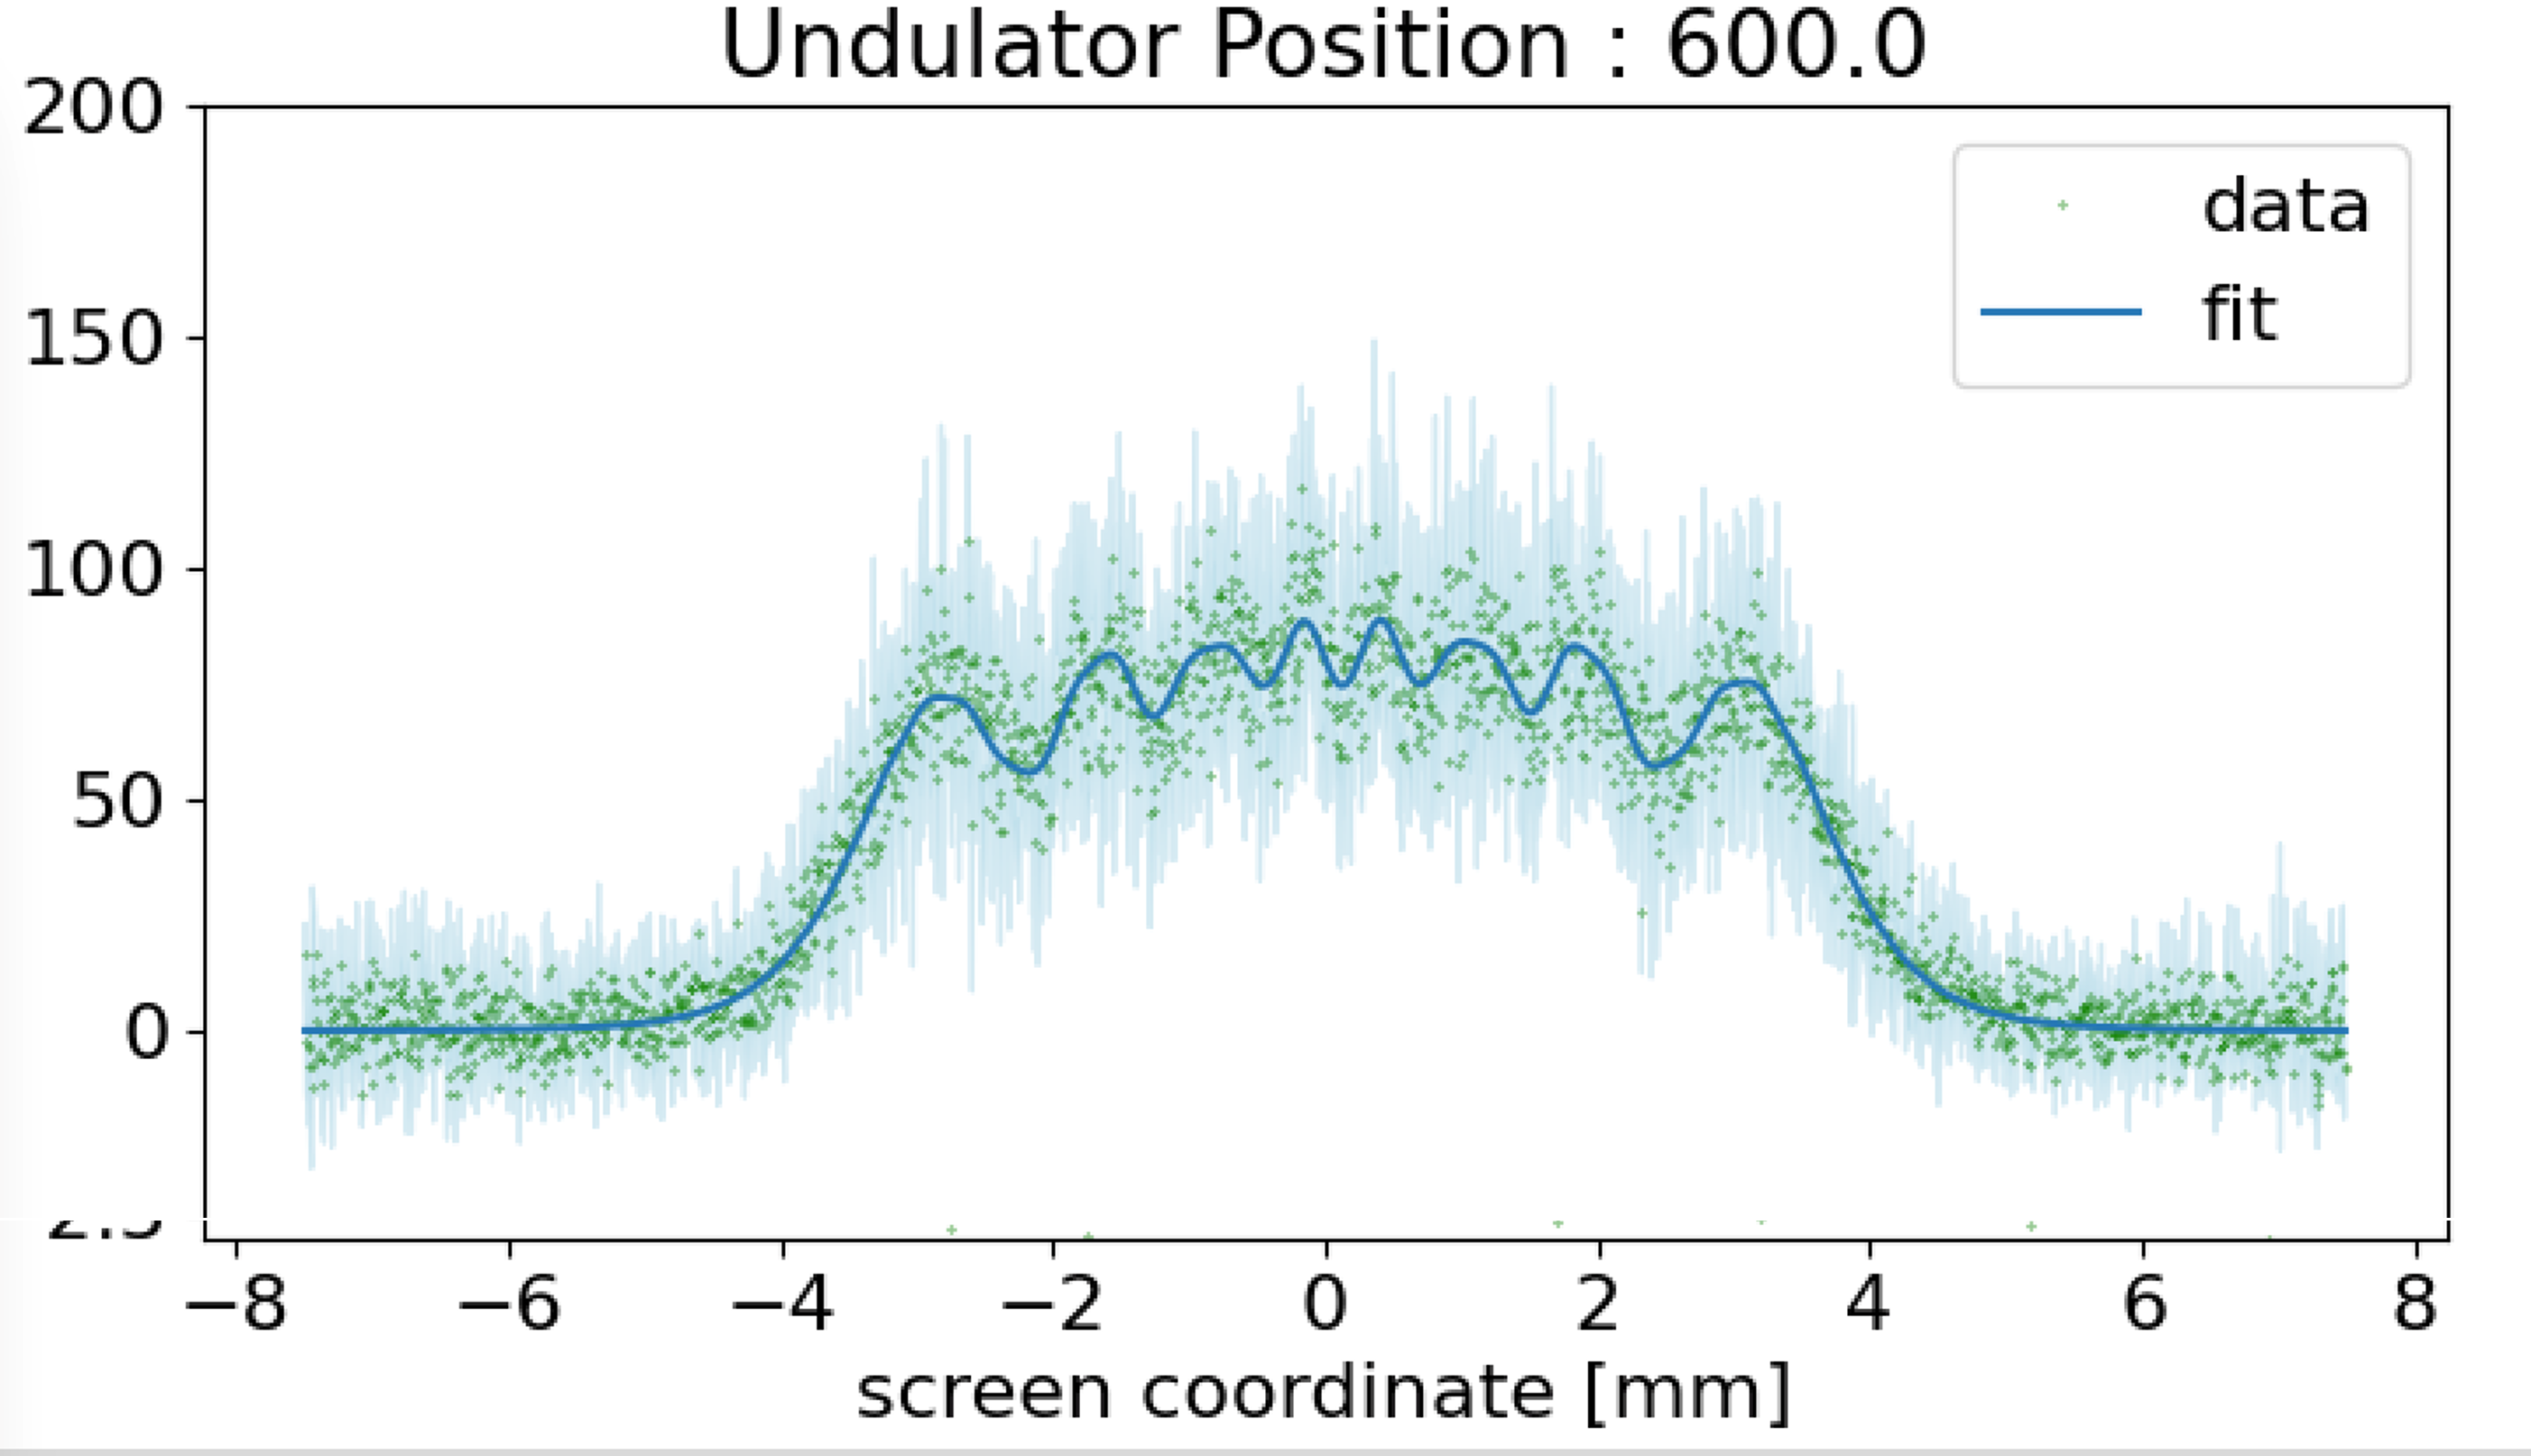
\includegraphics[width=\linewidth]{image/4-double_600.png}
    \subcaption{$d$=600~mm}
  \end{subfigure}
  \caption[2台のアンジュレータのデータ]{2台のアンジュレータのデータの回折パターンのフィッティングを示す。}\label{fig:double}
\end{figure}

\begin{table}[H]
\centering
\begin{tabular}{c|ccc}
  パラメータ & 初期値 & 最適値 &統計誤差(ブートストラップ)\\ \hline
  $\gamma$  & 381 & 381.197 & 0.0383\\
  $K$       & 0.971(固定) & - & -\\
  $\sigma_y$& 50~$\mu$m (固定) & - & -\\
  $z(U1-slit)$ & $z(U1-slit)$ + 1.38~m & - & -\\
  $z(U2-slit)$ & 10.26~m& 10.487~m & 0.035~m\\
  $z(slit-cam)$ & 4.11~m & 4.201~m & 0.006~m\\
  $w(slit)$ & 3~mm & 3.07~mm & 0.001~mm\\
  $y(beam)$ & 0.21~mm & 0.209~mm & 0.005~mm\\ 
  $y(slit)$ & 0.15~mm & 0.148~mm & 0.005~mm\\
  $\delta d$& 0~m & 0.033~m & 0.0005~m\\
  $ampl$    & 30 & 22.39 & 0.05\\ \hline
  $\chi^2$/ndf & 1.02 &  & \\ 
\end{tabular}
\caption[2台のアンジュレータのフィットパラメータ]{2台のアンジュレータデータに対する解析のフィットパラメータ}
\label{tab:double}
\end{table}
  
\section{統計誤差の見積もり}
\noindent \textbf{\underline{解析}}\par
統計誤差の見積もりはブートストラップ法によって行う。
ブートストラップ法はデータから復元抽出を行い、その復元抽出データから統計量を計算することで統計量の分布を推定する手法である。
下流アンジュレータの位置$d$に関してランダムに復元抽出を複数回(原則として100回)行い、抽出されたデータの集合に対してフィッティングを行う。得られたパラメータの分布から統計誤差を見積もる。
これにより、フィッティングパラメータとして$\gamma$の統計誤差が求まり、エネルギー測定結果の統計誤差を評価することができる。
同時に他のパラメータの統計誤差やパラメータ間の相関を見積もることができる。

\noindent \textbf{\underline{結果}}\par
$E_{beam} =195$~MeVのデータについてブートストラップ法による統計誤差の見積もりの結果の一例を示す。100個の異なる復元抽出データから得られる
$\gamma$の分布を図\ref{gamm_hist}に示す。
\begin{figure}[h]
  \centering
  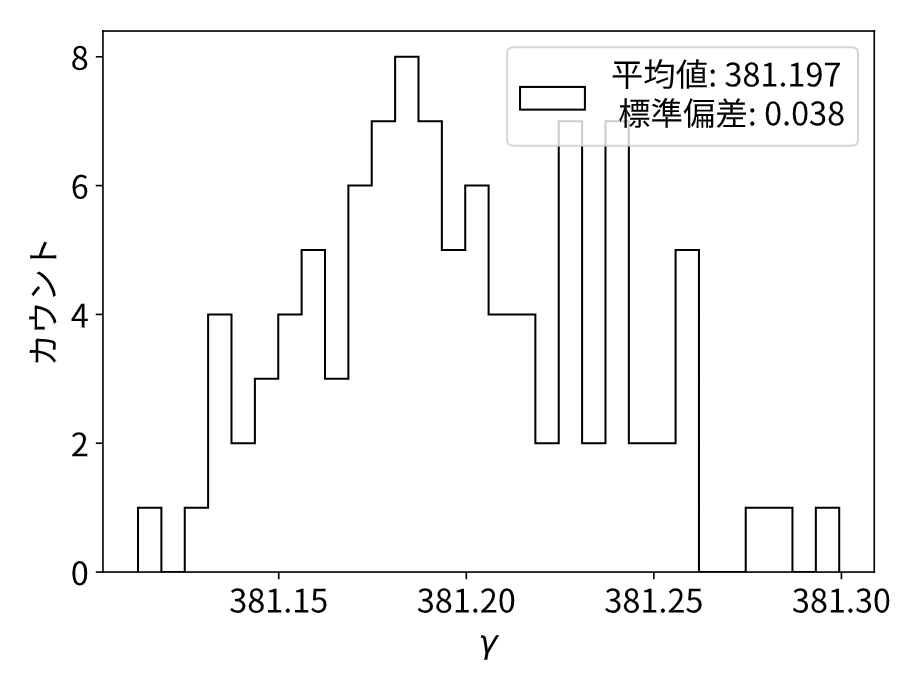
\includegraphics[width=0.8\linewidth]{image/4-gammahist.png}
  \caption[ブートストラップ法による$\gamma$の分布]{ブートストラップ法による$\gamma$の分布。100個の異なる復元抽出データから得られる$\gamma$の分布を示す。} \label{gamm_hist}
\end{figure}

この分布から求めた$\gamma$の平均値と標準偏差は
\begin{eqnarray}
  \gamma = 381.1972 \pm 0.0383
\end{eqnarray}
となり、$\lambda_L$ =404.656~nmにおける電子ビームエネルギーの統計誤差は10$^{-4}$の水準に達した。

各パラメータの誤差をブートストラップ法で見積もった結果を表\ref{tab:double}に示す。
また、$\gamma$と他のパラメータの相関は、$\delta d$を除いて相関係数0.1以下であった。$\delta d$と$\gamma$は図\ref{gamma_phase}に示すように強く相関しており
これはモデル関数の改良の余地があることを示唆している。
\begin{figure}[H]
  \centering
  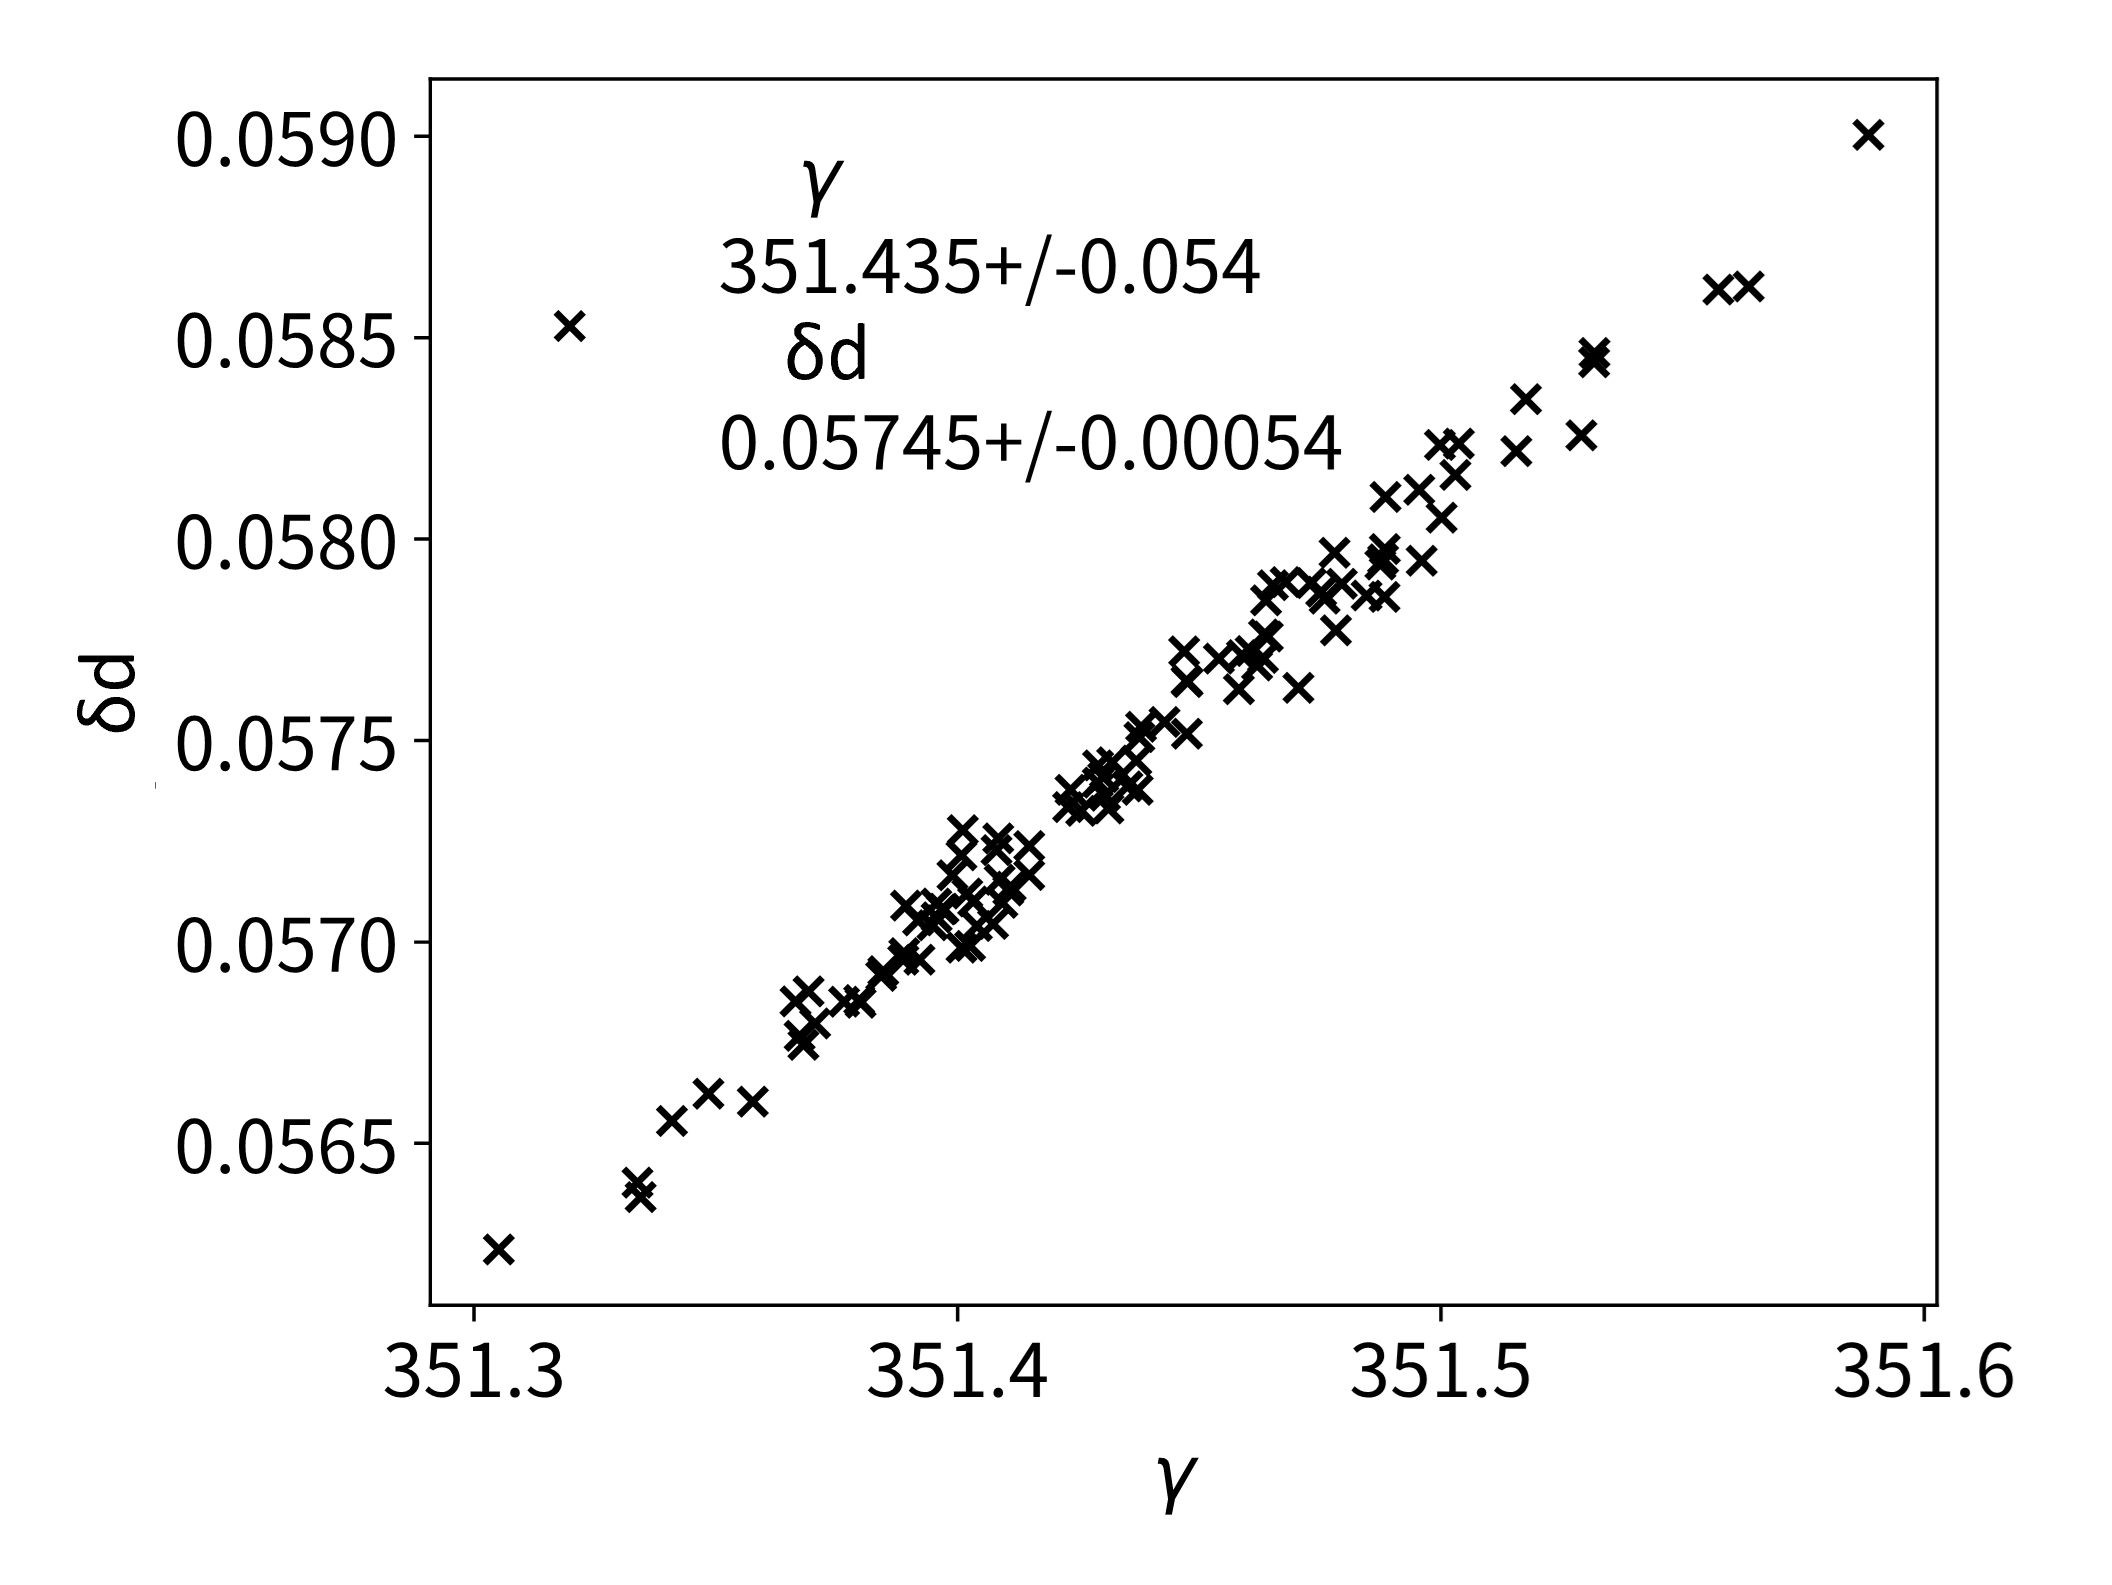
\includegraphics[width = 0.6\linewidth]{image/4-gamma_phase.png}
  \caption[$\gamma$-$\delta d$相関]{$\gamma$と$\delta d$のブートストラップ法による相関の見積もり。$E_{beam} =180$~MeVでの例を示した。プロットからわかるように
  $\gamma$と$\delta d$は強く相関している。}\label{gamma_phase}
\end{figure}

\section{系統誤差の見積もり}
波長依存性と位置依存性による誤差が主要な系統誤差の要因と考えられる。
\subsubsection{波長依存性}
\noindent \textbf{\underline{解析}}\par
前節で求めた較正波長(404.65 nm)におけるエネルギー測定の結果に加えて、同じモデル関数を用いて異なる波長でのデータからエネルギーを求める。
各波長に対してブートストラップ法を用いて統計誤差を見積もる。
異なる波長に対するエネルギーの分布から、モデル関数や装置のもつ波長依存性による系統誤差を見積もる。

\noindent \textbf{\underline{結果}}\par
横軸を波長に、縦軸をその波長における$\gamma$の推定値としたグラフを図\ref{wldep}に示す。
\begin{figure}[h]
  \centering
  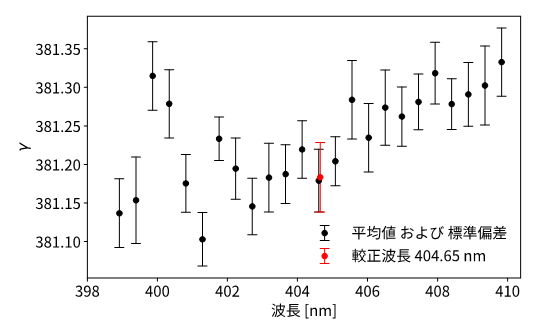
\includegraphics[width=0.8\linewidth]{image/4-wldep.png}
  \caption{エネルギーの推定値の波長依存性}\label{wldep}
\end{figure}

また、アクセプタンス全体における$\gamma_\lambda$の平均値および標準偏差は、
\begin{eqnarray}
  \gamma = 381.232 \pm 0.076
\end{eqnarray}
となった。この結果から波長依存性による系統誤差は$2\times10^{-4}$以下の水準であった。
この波長依存性の原因として、モデル関数の不完全性や光学系の非線形性が挙げられる。

以上の解析から195 MeVでのエネルギー測定の結果として
\begin{align}
  E_{beam} = 194.791 ~\pm 0.019(stat.) ~^{+0.056}_{-0.021}(syst.)~\text{MeV}
\end{align}
という結果を得た。

\subsubsection{位置依存性}
\noindent \textbf{\underline{解析}}\par
アンジュレータの位置によるエネルギーの推定値の違いを見積もる。
具体的には、アンジュレータの位置を4つの区間に分割し、各区間でエネルギーを求める。アンジュレータ位置に対する放射光関数の補正がどの程度の影響を持つかを見積もる。

\noindent \textbf{\underline{結果}}\par
横軸を4分割の区間のインデックス、縦軸を各区間で得られた$\gamma$の推定値としたグラフを図\ref{posdep}に示す。
\begin{figure}[H]
  \centering
  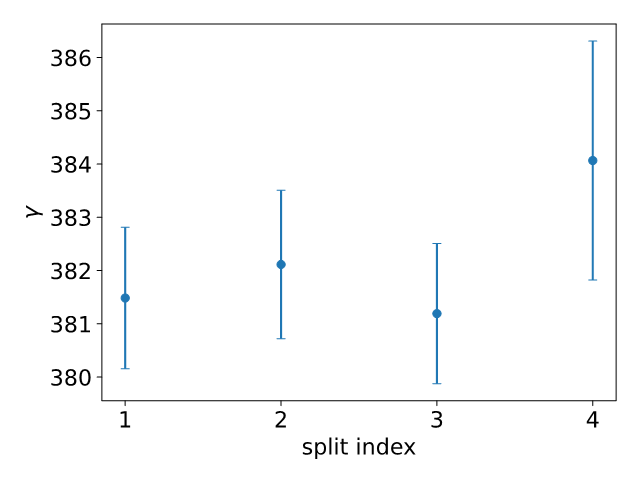
\includegraphics[width=0.8\linewidth]{image/4-posdep.png}
  \caption[アンジュレータ位置に対するエネルギーの推定値]{アンジュレータ位置に対するエネルギーの推定値。split index 1がもっとも上流であり、アンジュレータの可動範囲の最上流を0 mm としたときに
  split index 1は 0 mm から205 mm、split index 2は205 mmから410 mm、split index 3は415 mmから620 mm、split index 4は620 mmから825 mmの範囲を示す。}\label{posdep}
\end{figure}
元のデータよりも小さいデータでブートストラップを行ったため、各々の統計誤差は大きくなっている。
またsplit index 4のデータは特に統計誤差が大きい。これは2台のアンジュレータ同士の距離が離れた結果、放射光の振幅、位相関数の差が大きくなり、干渉光のずれの影響が大きくなるためだと考えられる。
単独アンジュレータのより詳細な解析によってこの位置依存性のずれは補正できる可能性がある。

\subsubsection{エネルギー依存性}
180、195、210 MeVの3つのエネルギーの結果の一例を表\ref{energy_dep}に示す。
\begin{table}[H]
  \centering
\begin{tabular}{c|ccc}
  エネルギー[MeV] & $\gamma$ & 統計誤差 & 系統誤差(波長依存性由来)\\
  \hline
  180 & 351.435 & 0.054  & 0.070\\
  195 & 381.197 & 0.038 & 0.076\\
  210 & 410.392 & 0.067  & 0.078\\
\end{tabular}\caption{エネルギーごとの決定精度}\label{energy_dep}
\end{table}
どのエネルギーにおいても統計誤差は$2\times10^{-4}$に収まっている。

また180 MeVと210 MeVにおける波長依存性の結果を図\ref{wldep_180210}に示す。
\begin{figure}
  \begin{subfigure}[h]{0.45\linewidth}
    \centering
    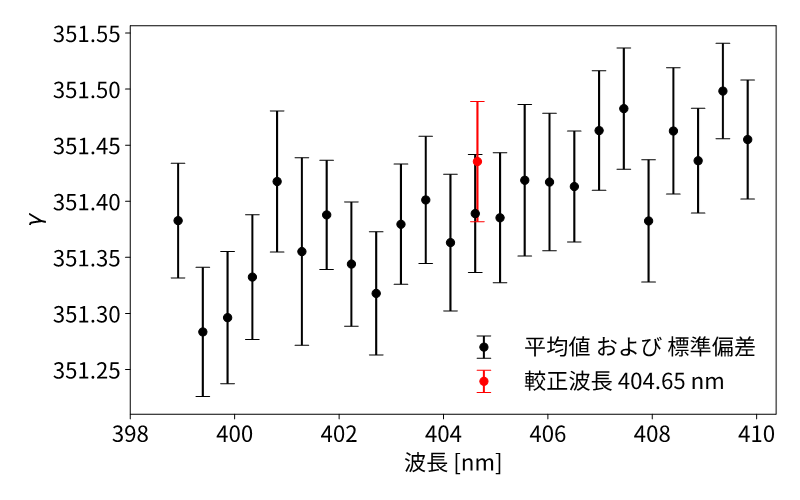
\includegraphics[width = \linewidth]{image/4-wldep180.png}
    \subcaption{180 MeV}
  \end{subfigure}
  \begin{subfigure}[h]{0.45\linewidth}
    \centering
    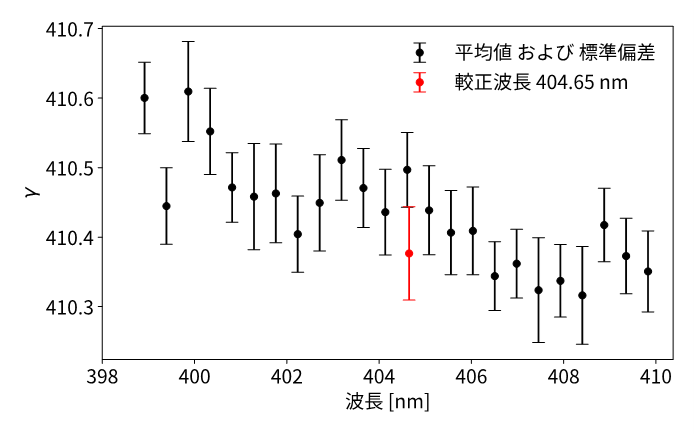
\includegraphics[width = \linewidth]{image/4-wldep210.png}
    \subcaption{210 MeV}
  \end{subfigure}
  \caption{180 MeVと210 MeVにおける波長依存性の結果}\label{wldep_180210}
\end{figure}
\ref{wldep}の195 MeVの結果と合わせて比較すると、180 MeVと195 MeVにおいては長波長側でエネルギーが大きくなる傾向があるのに対して、
210 MeVでは短波長側でエネルギーが大きくなる傾向があることがわかる。これは、210 MeVでは400 nm領域が共鳴波長の360 nmから外れているために
210 MeVだけが異なる振る舞いをしていると考えられる。
\end{document}